\documentclass[english,5p,authoryear]{elsarticle}
%\documentclass[11pt]{article}
\usepackage[utf8]{inputenc}
\usepackage[T1]{fontenc}
\usepackage{hyperref}
\usepackage[authoryear]{natbib}
\usepackage{textcomp}
\usepackage[font=footnotesize,skip=3pt]{subcaption}
\usepackage{graphicx}
\usepackage{fancybox}
\usepackage{xcolor}
\usepackage{makeidx}
\usepackage{float}
\usepackage{amsmath,amssymb}
\usepackage{eurosym}
\usepackage{setspace}
\usepackage{enumitem}
\usepackage{dsfont}

\PassOptionsToPackage{normalem}{ulem}
\usepackage{ulem}
\usepackage[toc,page]{appendix}
\usepackage{array,multirow,makecell}
\usepackage[switch,modulo]{lineno}
\renewcommand{\arraystretch}{0.8}
\setcellgapes{1pt}
\makegapedcells
\renewcommand*\thetable{\Roman{table}}
\renewcommand{\floatpagefraction}{0.80}
%\renewcommand{\footnotelayout}{\setstretch{0.5}}
\newcolumntype{R}[1]{>{\raggedleft\arraybackslash }b{#1}}
\newcolumntype{L}[1]{>{\raggedright\arraybackslash }b{#1}}
\newcolumntype{C}[1]{>{\centering\arraybackslash }b{#1}}

\setcounter{topnumber}{3}
\setcounter{bottomnumber}{3}
\setcounter{totalnumber}{4}

\usepackage{fancyhdr}
\pagestyle{fancy}
\fancyhf{}
\fancyhead[R]{\thepage}

%\usepackage[left=2.2cm,right=2.2cm,top=2.5cm,bottom=2.5cm]{geometry}
%\linespread{1}
%\date{}
\hypersetup{citecolor=blue,colorlinks=true}
\usepackage{cuted}
%\setlength{\parindent}{1pt}

\makeatletter
\def\ps@pprintTitle{%
 \let\@oddhead\@empty
 \let\@evenhead\@empty
 \def\@oddfoot{\@date}%
 \let\@evenfoot\@oddfoot}
\makeatother

\linespread{1}\selectfont

\begin{document}
\sloppy

\date{$\textnormal{\today}$}

\begin{frontmatter}{}
%%TC:ignore
  \title{French Attitudes on Climate Change, Carbon Taxation and other Climate Policies
  %French Attitudes over the Carbon Tax and other Climate Policies
%  \footnote{\scriptsize } % acknowledgments  
  }

% Done: si on vire la partie sur CC, effectivement on peut remplacer par .. over the Carbon Tax and other Climate Policies

%\author{Thomas Douenne and Adrien Fabre\thanks{}} 
\author[1]{Thomas Douenne}
\ead{thomas.douenne@psemail.eu}
\author[1]{Adrien Fabre\corref{cor1}}
\ead{adrien.fabre@psemail.eu}
\cortext[cor1]{Corresponding author}
\address[1]{Paris School of Economics; Université Paris 1 Panthéon-Sorbonne. 48 Boulevard Jourdan, 75014, Paris, France.}


\begin{abstract}
This paper aims to assess the prospects for French climate policies after the Yellow Vests crisis halted the planned increase in the carbon tax. From a large representative survey, we elicit knowledge, perceptions and values over climate change, we examine opinions relative to carbon taxation, and we assess support for other climate policies. Specific attention is given to the link between perceptions of climate change and attitudes towards policies. The paper also studies in detail the determinants of attitudes in terms of political and socio-demographic variables. Among many results, we find limited knowledge but high concern for climate change. We also document a large rejection of the carbon tax but majority support for stricter norms and green investments, and reveal the rationales behind these preferences. Our study entails policy recommendations, such as an information campaign on climate change. Indeed, we find that climate awareness increases support for climate policies but no evidence for the formation of opinions through partisan cues as in the US, suggesting that better access to science could foster support for climate policies.
\end{abstract}
% : modifier à la fin => ça me paraît bien

% Done : ("studies in details" -> "studies in detail")

% Done : ("better access to science could foster support for the ecology." -> "better access to science could foster support for climate policies.") -> should we put "ambitious climate policies"? => non

% Indeed, knowledge, perceived danger and support for policies are all positively correlated, suggesting that better access to science could foster support for the ecology, as we find no evidence for the formation of opinion through partisan cues as in the US.

% Un résultat clef de l'article est aussi l'importance de l'adhésion au mvt des GJ, et donc indirectement : la confiance dans le gvt, le partage équitable des efforts, et le déploiement des alternatives (dont l'absence revient aussi comme une barrière importante à surmonter). Pour le dire de manière plus brève, on pourrait simplement dire qu'on identifie les déterminants du rejet de la taxe carbone en France, et les attentes des citoyens en matière d'écologie.


%%%  éditeur :

% 1. (done) réduire (si possible) la taille de l'article -> gains d'espace possible dans la partie 3, mais perte d'espace avec la revue de littérature supplémentaire de l'intro. Aussi, suppression de la partie gaz de schiste => arf l'espace était mieux utilisé avec cette partie 3 je trouve, tant pis

% 2. (done ??) Please carefully check your highlights. They include typos, grammar mistakes and are not expressed in good English language. -> rien qui ne me saute aux yeux, à faire relire par un anglophone pour identifier ce qui ne va pas. La police des highlights ne rend pas super dans le PDF, à modifier aussi (ou éventuellement refaire en latek pour homogénéiser avec le texte).

% 3. (done ??) Please thoroughly check the whole manuscript regarding English language and precision of terms. For example, the last sentence of the abstract does not really make sense in relation to the topic of your paper: what do you mean by: “…could foster support for ecology.”? Wrong translation? Your focus is climate policies, not ecology. (done for "the ecology", but check the rest of the manuscript)

% 4. (done) Your references section needs careful checking. Many references are incomplete, e.g., volumes and page numbers missing for journal papers. -> j'ai changé le package, on peut aussi en prendre un autre, et il faut encore nettoyer certains éléments des références. => done

% 5. Footnote 5 is strangely separated in two parts. -> check this at the very end (peut changer pendant la mise en page)

% 6. (done ??) Please carefully follow the journal’s guidelines for the resubmission of revised manuscripts, available online as part of the Guide for Authors. -> il a l'air un peu tatillon, il faudra suivre ça à la lettre.


%%%  reviewer 1:

% 1. Réduire ou supprimer la partie 3, et de manière générale réduire le nombre de tableaux et de graphiques du papier. La contribution de cette section n'est pas évidente pour lui, parce qu'on donne beaucoup de résultats sans indiquer clairement ce que l'on cherche à montrer, et parce que cela a déjà été fait ailleurs dans la littérature. Il pense que notre contribution se situe dans les sections 4 à 6, lesquelles pourraient être complétées. -> c'est la première chose qu'on va devoir déterminer, que faire de cette partie 3 ? Une option est de la supprimer, en passant les graphiques en online appendix, et en donnant les principaux résultats dans les autres parties, notamment la partie 6 lorsqu'on met en relation connaissances/opinions sur el CC et choix de politiques.

% 2. (almost done) Revoir la conclusion pour davantage résumer nos résultats, et répondre à la question "So what does it all mean?". -> actuellement on passe direct aux implications pour les politiques climatiques, peut-être devrait-on faire un pas en arrière et essayer d'abord d'expliquer le sens de ces résultats ? Pour le moment je ne suis pas très inspiré.

% 3. (done ? référence supprimée, mettre ailleurs ?) Eviter de finir le papier avec une comparaison avec la Suède. Déplacer cela ailleurs (le reviewer trouve cela étrange d'écrire un papier sur la France et de finir par la Suède). -> Le 2e reviewer trouve cette phrase bancale, donc à changer de toute façon.

% 4. (done) Tester la pertinence de nos indices (scores), par exemple en estimant le Cronbach alpha des éléments inclus (Cf. Hoppe, I., Taddicken, M., & Reif, A. (2018). What do people know about climate change — and how confident are they? On measurements and analyses of science related knowledge. Journal of Science Communication (Jcom), 17(3): A01, pp. 1-26. doi:10.22323/2.17030201.). -> Pour les connaissances CC, on obtient un alpha de 0.32, et en enlevant la variable emission_cible on passe à 0.38 mais c'est toujours loin de 0.7. Explications possibles : léger aléatoire des questions de connaissances (notamment la cible d'émissions) qui fait mécaniquement décroitre alpha, et multi-dimensionalité des connaissances (scientifiques, impacts, lien avec le quotidien) qui est justement la raison pour laquelle nous avons varié les questions. L'alpha de Cronbach n'est que moyennement pertinent dans notre cas, sa faible valeur rejette juste l'hypothèse que les connaissances en matière de CC peuvent être mesurées sur une échelle unidimensionnelle.
% -> La référence donnée par le relecteur est très intéressante et on pourrait citer ce papier (ou Kiel & Rost 2002, voir aussi Tobler et al 2012) pour expliquer que nos questions cherchent à capturer les différentes dimensions de connaissances (qui correspondent à leurs catégories). Ils calculent le alpha par catégorie de connaissances, et non sur la somme de ces diverses dimensions. On peut difficillement faire un tel exercice avec nos données car nous n'avons pas assez de questions par catégorie, ce qui implique un alpha proche de 0. Le mieux que l'on peut faire est peut-être de tester différentes manières de construire l'indice en online appendix, montrer une table des corrélations entre les différentes dimensions (i.e. différentes composantes de l'indice).
% Il exprime aussi des doutes vis-à-vis de l'inclusion de l'Inde dans le score "connaissances". -> la variable Inde n'a pas d'effet sur la valeur de alpha, mais on pourrait tester la sensibilité sur les résultats.

% 5. (done) Style: better avoid „to do so“ 2x in one paragraph of the introduction.

% 6. (done) Line 56: You write that France “recently experienced a carbon tax increase”, although before you said it was planned but canceled. Is this contradictory?  => "On the one hand, the protestof the Yellow Vests that originated in November 2018 against the planned doubling in the carbon tax  — from 44.6 to 86.2e/tCO2 in 2022 — led the government to halt the increasing trajectory" + "that started at 7e/tCO2 in 2014." au début. Si ça n'est toujours pas assez clair il nous dira et on remplacera la fin incriminée par "experienced a large debate over carbon taxation".

% 7. (done) The term “primings” in Figure 1 is unclear. -> soit on l'explique dans le texte, soit on le supprime de la figure. Etant donné la nécessité de raccourcir le papier, je penche plutôt pour la 2e option puisqu'on n'exploite pas cette partie du sondage dans ce papier. => ok, on peut remplacer par "Set up, households characteristics" (note la , au lieu de : pour rester techniquement véridique) -> Ok

% 8. (done) In Figure 3 and in the text you use the term “anthropic”. I would say the term “anthropogenic” is more common.

% 9. (done) Figure 8: “perceived responsible” sounds a bit odd. Perhaps better “responsibility”.  =>  "Entities perceived responsible for CC" ou "Perception of responsibility for CC". Pour le moment, la 1ere a été retenue.

% 10. (done) Figure 19: did nobody reply “insufficient”? Because I see no red bar. -> problème avec les couleurs dans la légende.

% 11. (done) Figure 24: What does “number of policies” mean here? -> clair avec le texte, mais si la figure doit être "self-contained" alors il faudrait effectivement préciser cet intitulé, soit avec une note en dessous, soit avec un intitulé plus long tel que "# of policies supported". => 2è option

% 12. (done but need to comment in text) Table 2: I kind of expected that you would also examine the determinants of the approval of carbon taxes with different revenue uses, probably in a separate table. But perhaps you have a reason why you did not do this. -> Done in online appendix, maybe need to comment it in the text. Note also that we already somewhat do it in a more synthetic way with our dependent variable "earmarking vs transfers".

% 13. (done) Final suggestion: Perhaps mention “carbon tax” somehow in the title. -> Ok: French Attitudes over the Carbon Tax and other Climate Policies


%%%  reviewer 2:

% 1. (done, mais à relire et bien vérifier citations) Faire une revue de littérature plus étendue en introduction (à partir de la ligne 44) plutôt que de la disséminer dans le texte (ref, probablement à citer aussi : https://www-tandfonline-com.inshs.bib.cnrs.fr/doi/full/10.1080/14693062.2019.1639490). -> Je ne suis pas très fan de cette suggestion, je préfère avoir toutes les références placées dans le texte là où elles sont pertinentes, plutôt que de faire une enième revue de littérature alors qu'il en existe déjà plein. Mais l'éditeur a malheureusement l'air d'y tenir...

% 2. (done) Utiliser anthropogenic plutôt qu'anthropic. 

% 3. (done) line 249: please define the concept of "warm glow" in this context -> cf. commentaire dans le texte. => cf. ma réponse -> ok pour la footnote, mais en section 5 puisque la 3 disparait du texte.

% 4. (done) line 570: "...are usually less cost-effective than Pigouvian taxes". There are situations in which this is not necessarily the case. See for example: Goulder, Hafstead, Williams 2016 General Equilibrium Impacts of a Federal Clean Energy Standard. If there are additional distributional constraints, other climate change policies might be also more efficient (Stiglitz, 2019, EER, already cited in your manuscript). -> cf. commentaire dans le texte.

% 5. page 11 Table I: - Why is "extreme left" not included in column (3) and (6)? - Please include Yellow Vests: opposed. This is quite an interesting variable and you also explicitly refer to it on page 12 in line 724. -> il s'agit des variables omises de la régression, je ne sais pas s'il n'a pas compris ou s'il suggère juste de ne pas mettre ces dummies comme variables omises. D'après sa remarque, je pencherai plutôt pour la 1ere explication même si ça me semble assez gros. => nan il a raison y a un problème, la variable omise pour Left-right c'est censé être Indeterminate. En fait c'est qu'on exclut les Indeterminate dans (3) et (6) à cause de l'interaction avec Diplome. Je crois qu'il faut rajouter une dummy Indeterminate x Diploma et remplacer NA par la moyenne de Left-right (numérique) pour les Indeterminate, comme ça on conserve tout l'échantillon. Pour Yellow Vests je penche pour l'explication qu'il préfère PNR comme modalité omise. On peut soit obtempérer, soit lui dire que ça fait sens d'omettre "oppose", qui est la plus extrême. -> Ok. Pour GJ je suggère de garder opposed parce que ça permet de mieux voir la différence avec les soutients

% 6. (done) line 869: There is more recent literature on trust and climate policy support. see for example Rafaty, R. (2018). Perceptions of Corruption, Political Distrust, and the Weakening of Climate Policy. Global Environmental Politics, 18(3), pp. 106-129. -> ref aussi donnée par Linus pour le premier papier (en complément d'Alesina et al). J'ai fait une proposition de modif dans le texte.

% 7. (done, except Cherry et al) line 883: please cite additional literature here. For example Ziegler, A. (2017) Political orientation, environmental values, and climate change beliefs and attitudes: An empirical cross country analysis. Energy Econ. 63, 144–153. Cherry, T. L., Kallbekken, S. & Kroll, S. (2017). Accepting market failure: Cultural worldviews and the opposition to corrective environmental policies. J. Environ. Econ. Manage. 85, 193–204. -> 1er article (Ziegler) pertinent pour une comparaison entre pays, notamment sur les limites du paradigme gauche/droite en dehors des Etats-Unis. Pour autant, on ne peut pas le citer à la suite de Drews & van den Bergh, il faut une citation à part car les conclusions sont plus spécifiques et ne vont pas dans le même sens. / 2e article (Cherry et al) assez nul dans lequel des étudiants échangent des jetons, je comprends pas que ça passe dans le JEEM. Pas très pertinent d'étudier l'importance des "worldviews" sur un échantillon d'étudiants américains, population peu hétérogène. Soit le relecteur est l'un des auteurs, soit il veut qu'on le cite parce que c'est dans le JEEM. Je suggère de le citer quand même pour ne froisser personne, mais l.883 ce n'est pas forcément le meilleur endroit du texte. La référence pourrait être glissée quelque part si on liste des papiers sur le sujet dans notre revue de littérature en intro. => 1: ok!; 2: arf ok.

% 8. (done) line 886-890: please refer to Table 2.3.

% 9. (done) line 946: What does "this policy" refer to - dividends or kerosene taxation or the combination? -> j'avoue que ce n'est pas clair du fait de la footnote qui fait référence à une taxe carbone non limitée au kérosène. J'ai fait une suggestion dans le texte mais on peut revenir dessus. => ça me paraît bien comme ça, il n'y a plus d'ambiguïté

% 10. (done except last point) Typos:
    % * (done) abstract: "studies in details" should be "studies in detail"
    % * (done) page 3 line 133: "it will severely effect" should be "affect"
    % * (done) line 329: "thought is was desirable" should be "it"
    % * (done) line 852: "consistently" should be consistent
    % * (done) line 861: "does not simply reflects from lower..." should this be "does not simply reflect lower" ?
    % * (done) line 885: "that people most likely" should be "that people that are most likely"?
    % * line 957-962: There is something wrong with this sentence and it also is too long. -> we should change it anyway given other reviwer's comment. 


\begin{keyword}
Climate Policy; Carbon tax; Preferences; Acceptability; France
\end{keyword}
%%TC:endignore
\end{frontmatter}{}

% \vspace*{2.3cm}

% \begin{strip}

% \linespread{1.5}\selectfont

% \begin{center}
%     {\Large \textbf{ 
%11


%%TC:ignore
%\paragraph*{\textbf{Disclaimer}} This is a work in progress. Please, do not cite without the authors' permission. % and, therefore, a draft version of the final paper. Please, do not cite without the authors' permission.

% Done: disclamer deleted

\paragraph*{JEL classification} D78; H23; Q54; Q58

%\paragraph{Word count} 7909 + 91 = 8000 words.

% Q54	Climate • Natural Disasters and Their Management • Global Warming
% Q58	Environmental Economics : Government Policy
% D78   Positive Analysis of Policy Formulation and Implementation
% H23	Externalities • Redistributive Effects • Environmental Taxes and Subsidies

% D72	Political Processes: Rent-Seeking, Lobbying, Elections, Legislatures, and Voting Behavior
% D91	Role and Effects of Psychological, Emotional, Social, and Cognitive Factors on Decision Making
% H31	Fiscal Policies and Behavior of Economic Agents : Households
% Q48	Energy : Government Policy
% Q52	Pollution Control Adoption and Costs • Distributional Effects • Employment Effects



%     }}
% \end{center}

% \vspace*{2cm}

% \begin{center}
% \textbf{Abstract:} 
% \end{center}

% \hfill \break
%\hspace*{1.6cm} \parbox{15cm}{\noindent {\textit{The objective of this paper is to assess the prospects for French climate policies after the Yellow Vests crisis halted the planned increase in the carbon tax. From a large representative survey, we elicit knowledge, perceptions and values over climate change, we examine opinions relative to carbon taxation, and we assess the support for other climate policies. Specific attention is given to the link between perceptions of climate change and attitudes towards policies. The paper also studies in details the determinants of attitudes in terms of political and socio-demographic variables. Among many results, we find limited knowledge but high concern for climate change. We also document a large rejection of the carbon tax but majority support for stricter norms and green investments. Our study entails policy recommendations, such as an information campaign on climate change. Indeed, knowledge, perceived danger and support for policies are all positively correlated, suggesting that better access to science could foster support for the ecology, as we find no evidence for the formation of opinion through partisan cues like in the US.}}}

%France has recently abandoned its planned increase of a national carbon tax due to a lack of public support, that culminated with the Yellow Vests movement. The objective of this paper is to assess the prospects for future climate policies after the Yellow Vests. From a large survey representative of the French population, we elicit both knowledge and values over climate change; we examine the perceptions specific to carbon taxation and the determinants of its rejection; we assess the support for other climate policies. A specific attention is given to the link between perceptions of climate change and attitudes towards policies. The paper also offers a detailed characterization of the heterogeneity in attitudes along political and socio-demographic variables.


%\vspace*{2cm}

% Carattini et al : D72, D78, H23, Q54 / acceptability, carbon pricing, carbon taxes, public support, revenue recycling

% \vspace{0.3cm}

% \end{strip}

% \clearpage
%\newpage


\setcounter{tocdepth}{2}
%\tableofcontents
%%TC:endignore

\vfill\eject 
%\linenumbers

\section{Introduction}

The French government is currently facing a two-sided challenge on climate policies. On the one hand, the protest of the Yellow Vests that originated in November 2018 against the planned doubling in the carbon tax  --- from 44.6 to 86.2\euro{}/tCO$_2$ in 2022 --- led the government to halt the increasing trajectory that started at 7\euro{}/tCO$_2$ in 2014. On the other hand, a large campaign called \href{https://laffairedusiecle.net/}{``Affaire du siècle''} started in December 2018 against its inaction for the environment, gathering over two millions signatories in a month. It is so far unclear how the tension between these two \textit{a priori} antagonistic objectives will be resolved. In particular, one may wonder whether the two movements involve distinct groups with opposite interests, or rather reflect a commonly perceived inadequacy of the solution proposed by the government to address the climate threat.

%This paper aims to understand French perceptions over both climate change (CC) and the policies that should be implemented to tackle it.

This paper aims to understand French perceptions over the carbon tax and other climate policies. It builds on a new survey conducted on a sample of 3,002 respondents representative of the French population. Our survey contains questions to assess respondents' knowledge about climate change (CC) and their perceptions over its causes and consequences. As the paper was primarily motivated by the failed attempt to increase the French carbon tax, we examine in detail attitudes towards this instrument. We propose to respondents a Tax \& Dividend policy, i.e. a carbon tax whose revenue would be returned lump-sum uniformly to all adults. This policy differs from the one proposed by the government, since the revenue would have been used to fund the general budget instead. We identify respondents' expected winners and losers, and the perceived problems and benefits of this instrument. We devote particular attention to the issue of mobility that appears critical in the current debate. We then turn to the support for a carbon tax with alternative uses of the revenue, such as more targeted transfers, earmarking, and double-dividend strategies. We also study the support for other climate policies, including norms and other Pigouvian taxes, and local policies for urban transport. Finally, we identify the determinants of attitudes over both climate change and climate policies, as well as the link between the two.
% DONE: ", and the timing of its effects" -> ""
% : slighlty change the focus wrt CC. => Suggestion (too long but something like this) "Our survey contains questions to assess" -> To grasp the extent of concern about climate change (CC) and the willingness to tackle it, our survey assesses -> On dit que c'est ok comme ça, on ne change rien ? => oui

% Done : ("To do so, we conducted a new survey on a sample of 3,002 respondents representative of the French population" -> "It builds on a new survey conducted on a sample of 3,002 respondents representative of the French population") -> "on a sample" ou "over a sample"? => on
% Done : ("To do so, we propose" -> "We propose")

% DONE: we show that French people have biased beliefsover carbon tax properties, but .. ->  we show that French people reject the carbon tax because of biased beliefs over its properties, but..
For a general presentation of attitudes over climate change, we suggest \citet{whitmarsh_2_2018}, while for a more specific review on their trends and determinants, we redirect to \citet{brechin_public_2010} and \citet{ziegler_political_2017}. Our paper contributes mainly to a growing literature on the political economy of climate policies. As an entry point to previous related studies, refer to \citet{maestre-andres_perceived_2019} who review the perceptions of climate policies, \citet{drews_van_der_bergh_2016} who review the determinants of their support, and to \citet{carattini_overcoming_2018} for a comprehensive overview on attitudes over the carbon tax. 
% DONE: added paragraph above (pour caser le CC hors d'une footnote) and removed  \citep[see][for a comprehensive review]{carattini_is_2018}

% DONE: "As carbon taxation is often considered by economists as the cornerstone of climate policies, it is no surprise that the literature has to a large extent focused on this instrument. Using a post-electoral survey, \citet{thalmann_public_2004} analyzes the determinants of opposition towards carbon taxation in Switzerland. Among other results, he finds that political leaning, education and self-interest are correlated with acceptance." -> "A large extent of the literature has focused on the carbon. Using a post-electoral survey in Switzerland, \citet{thalmann_public_2004} finds that political leaning, education and self-interest are correlated with acceptance."
A large extent of the literature has focused on the carbon tax. Using a post-electoral survey in Switzerland, \citet{thalmann_public_2004} finds that political leaning, education and self-interest are correlated with acceptance. Subsequent literature has confirmed the importance of self-interest \citep[e.g.][]{fischer_et_al_2011,baranzini_effectiveness_2017} although \cite{kallbekken_saelen_2011} find that perception of the tax' effectiveness and its distributive properties play a larger role in Norway. The critical role of the tax' effectiveness has been confirmed by numerous contributions that pointed out the higher acceptance of taxes whose revenue was earmarked towards green investments \citep[e.g.][]{saelen_kallbekken_2011,baranzini_effectiveness_2017}. Similarly, studies have confirmed that people tend to prefer more progressive schemes \citep{brannlund_tax_2012,gevrek_public_2015} and more targeted revenue recycling \citep{kallbekken_et_al_2011}. In a companion paper \citep{douenne_can_2019} based on the same survey, we show that French people reject the carbon tax because of biased beliefs over its properties, but if convinced about their own gain, the environmental effectiveness and the progressivity of the mechanism, they would largely approve it. Among the potential barriers to the implementation of carbon taxation, \citet{kallbekken_aasen_2010} emphasize the importance of the availability of alternatives to fossil fuels. When these alternatives are lacking or not easily affordable, carbon taxation is perceived as just a pretext to increase taxes \citep{dresner_social_2006,klok_et_al_2006}. Finally, as shown by \citet{harring_jagers_2013}, trust in politicians is also a key factor for carbon tax acceptance, which relates to the recent findings of \citet{rafaty_perceptions_2018} who shows that higher political distrust is associated with weaker climate policies.
% "large distributive effects" ou "a higher burden on the poors".
% useless and only a pretext -> as just a pretext
% DONE: suppression de "In a recent study, \citet{anderson_can_2019} show that in the U.S. attitudes towards carbon tax are largely driven by ideology. This result echoes the findings of \citet{cherry_accepting_2017} who show that people tend to reject corrective policies that would improve their welfare, and that this rejection is largely correlated with their worldviews. , puisqu'on cite Cherry juste en-dessous et Anderson ailleurs dans le texte

% DONE: removed "\citet{drews_van_der_bergh_2016} and \citet{maestre-andres_perceived_2019} review the literature to identify the determinants of the support for climate policies."
While a lot of attention has recently been put on carbon taxation, fewer studies have investigated attitudes towards other climate policies. Yet, as highlighted by \citet{stern_report_2017} and \citet{stiglitz_addressing_2019} a single price instrument may not be the best response to climate change in a second-best world. The main factors driving people's preferences between various policies appear to be their degree of coercion, the behavior targeted by the policy \citep{de_groot_schuitema_2012}, and the perceived cost. It follows that subsidies are in general preferred over taxes \citep[e.g.][]{tobler_et_al_2012,cherry_accepting_2017}, and more voluntary measures over hard regulations \citep{attari_et_al_2009}. The present paper contributes to the literature by providing a comprehensive analysis of perceptions and attitudes towards CC, carbon taxation and other climate policies in a country that has recently experienced a carbon tax increase and a large debate ensuing. As it is based on an unusually large sample representative of the French population, the paper also goes further than previous studies in identifying the heterogeneity in people's attitudes over climate policies. % DONE: dernière phrse + footnote peut-être en trop, mais je ne sais pas trop ou caser ça. => DONE: virer l'avant-dernière phrase* (redite), dans celle d'avant dire CCCP au lieu de CP (pour la transition), et passer la footnote dans le texte: ce sont des papiers importants
% *  It also investigates the determinants of perceptions of climate change, and documents the link with attitude towards climate policies.

% DONE : regarder ce papier proposé par le 2e relecteur, et le citer si pertinent => oui ça vaut le coup, contrairement au papier de 2016, ils ne regardent pas l'influence des perceptions CC. je l'ai inséré au début https://www-tandfonline-com.inshs.bib.cnrs.fr/doi/full/10.1080/14693062.2019.1639490

%As an entry point to previous related studies, please refer to \citet{drews_van_der_bergh_2016} who review the determinants of the support for climate policies and to \citet{carattini_overcoming_2018} for a comprehensive overview on attitudes over the carbon tax. For a general presentation of attitudes over climate change, we suggest \citet{whitmarsh_2_2018}, while for a more specific review on their trends and determinants, we redirect to \citet{brechin_public_2010}. The present paper contributes to the literature by providing a comprehensive analysis of the determinants of attitudes about climate change and climate policies in a country that has recently experienced a carbon tax increase and a large debate ensuing.

Section \ref{sec:survey} presents the survey. Section \ref{sec:attitudes_climate_change} describes attitudes towards climate change. Section \ref{sec:attitudes_carbon_tax} focuses on tax \& dividend policies, its perceptions, and the reasons explaining the low support for this policy. Section \ref{sec:attitudes_other_policies} studies the support for alternative revenue recycling mechanisms as well as for other climate policies. Section \ref{sec:determinants} examines the heterogeneity in attitudes expressed in the previous sections and characterize their determinants. Section \ref{sec:conclusion} concludes. Finally, further material can be found in appendix and online Appendix.

% DONE : ajouter quelque chose comme : "Further material can be found in appendix, and alternative specifications and robustness tests are gathered in an online appendix." => DONE en + court, cf. ci-dessous

%\footnote{The French carbon tax was introduced in 2014 at 7\euro/tCO$_\textnormal{2}$ and increased to attain 44.6\euro/tCO$_\textnormal{2}$ in 2018. While it was supposed to continue growing to reach 86.2\euro/tCO$_\textnormal{2}$ by 2022, the trajectory stopped in November 2018 following the Yellow Vests' protests.}

% Done : éclaircissement sur l'historique de la taxe (pour préciser que des augmentations ont bien eu lieu avant l'abandon).

% Since France recently experienced a large debate over the carbon tax, the issues covered in the survey are not hypothetical questions but refer to policy discussions that people are aware of. The paper also contributes to the literature by providing a comprehensive analysis of the political and socio-demographic determinants of perceptions about climate change and climate policies, and how the former may affect the latter.


\section{The survey}\label{sec:survey}

    \subsection{Presentation of the survey}

We collected 3002 responses in February and March 2019 through the survey company Bilendi. This company maintains a panel of French respondents to whom they can email survey links. Respondents are
paid 3\euro{} if they fully complete the survey. The respondents who choose to respond are first filtered through some screening questions which ensure that the final sample is representative along six socio-demographic characteristics: gender, age (5 brackets), education (4), socio-professional category (8), size of town (5), and region (9). The quotas are relaxed by 5\% to 10\% relative to actual proportions. Table \ref{tab:Sample-Characteristics} in Appendix \ref{app:Raw-Data} shows that our sample is still extremely representative. Nonetheless, observations are weighted to correct small differences between sample and population proportions. The median time for completion of the survey was 19 minutes. 

The full survey in French can be seen \href{http://preferences-pol.fr/doc_q.php#_e}{online},\footnote{\href{http:\/\/preferences-pol.fr\/doc\_q.php\#\_e}{preferences-pol.fr/doc\_q.php\#\_e}} the questions analyzed are translated in Appendix \ref{app:questionnaire}, and the code is available on \href{https://github.com/bixiou/beliefs_climate_policies}{github}. Figure \ref{fig:survey} presents in a diagram the sequence of  questions.

\begin{figure}[!htbp]
\centering
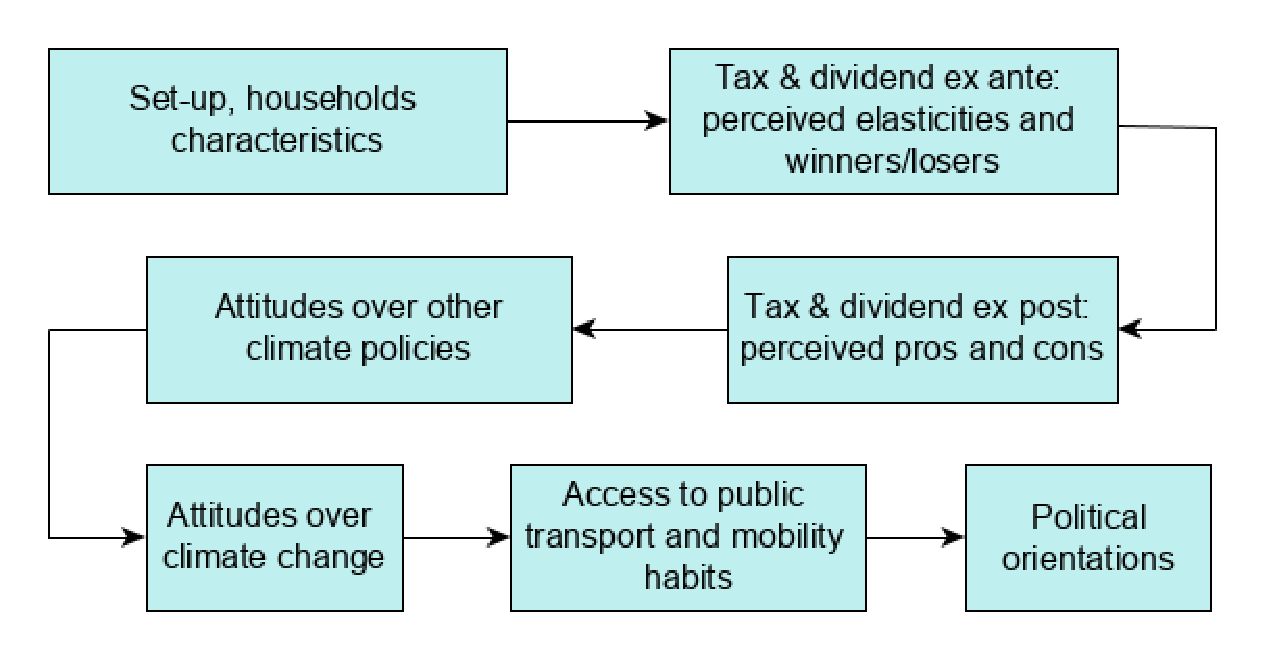
\includegraphics[width=\columnwidth]{Images_EPS/diagram_survey_attitudes.eps}
\caption{Diagram of the sequence of questions.}
\label{fig:survey}
\end{figure}
% DONE energies -> energy
% with a priming where information on climate change or on particulate matter is randomly displayed or not. This priming divides the sample in four groups, who receive either one block of information, the other, none or both of them. Then, we ask 
% motivate why tax & dividend
The survey starts by asking for households' socio-demographics and energy usage. The distribution of answers are much in-line with official statistics, as shown in Table \ref{tab:app-energetic-characs} in Appendix \ref{app:Raw-Data}. Then, we describe Tax \& Dividend reforms where the revenues of an increase in the French carbon tax by 50\euro{}/tCO$_\textnormal{2}$ are redistributed uniformly to all adults. We first allocate respondents randomly to a sectoral Tax \& Dividend reform, which concerns either gas and domestic fuel (i.e. housing energy), or gasoline and diesel (i.e. transportation energy). Respondents are asked to estimate their reaction to price changes, the reaction of French people, and how much purchasing power they would gain or lose from the policy. To this end, exact price variations and the amount transferred are provided, and respondents can choose among answers given in different brackets. Then, we study perceptions and support for a Tax \& Dividend on both sectors combined, before and after providing new information to the respondents. This new information is either that the policy is progressive, or whether their household would win or lose some purchasing power through the reform. Before providing information, we let respondents pick the categories of losers and winners from the reform; and after the information, they choose the benefits and the problems associated with this reform. We study these perceptions of the policy in the present paper, but please refer to our companion paper \citep{douenne_can_2019} for details and analyses on the other questions about Tax \& Dividend reforms. % %and where respondents are asked to estimate their own elasticity as well as that of French people. To this end, we borrow the phrasing of \citet{baranzini_effectiveness_2017}, and ask the expected decrease in consumption that would follow a 30\% increase in the price of heating (or equivalently, an increase of 0.50\euro{} per liter in fuel prices), among 5 brackets. 

% The survey starts by asking for households characteristics. In addition to the quotas strata, socio-demographic characteristics include zip code, household structure, income of the respondent and of their household. Energetic characteristics contain surface of accommodation, heating type (collective or individual) and energy source; as well as the number of vehicles, type(s) of fuel, distance traveled last year and average fuel economy. The distributions of answers are much in-line with official statistics, as shown in Table \ref{tab:app-energetic-characs} in Appendix \ref{app:Raw-Data}.

    \subsection{Eliciting attitudes} % towards climate change and climate policies} DONEw: raccourci


After inquiring about the support for Tax \& Dividend, we ask respondents to assess on a Likert scale different ways to recycle the revenues of a carbon tax. On another Likert scale, we examine opinions on other climate policies, notably new norms or Pigouvian taxes. We then measure respondents' knowledge about climate change by asking for its origin (anthropogenic or natural), its causes (in terms of gases and activities), which region it will most affect (between India and the European Union), and what reduction of emissions is needed by 2050 to respect the +2\textdegree{}C target. At the same time, we assess attitudes over climate change by asking respondents about the frequency with which they talk about it, the gravity of its consequences, the generations it will severely affect, and the entities responsible for its occurrence. We continue by surveying if and how climate change influences one's decision to have a child, under which conditions one would be ready to change their lifestyle to fight climate change, and whether one would be ready to adopt a sustainable lifestyle if policies were aligned to this goal. We also ask questions about diesel taxation. Then, we evaluate the respondents access to public transport, their mobility habits, and if there is room for changing these habits. Finally, we ask for their political preferences, including their positioning in relation to the Yellow Vests. The survey ends with a text box where the respondents can leave a comment.
% Done : ("severely effect" -> "severely affect")
% Done : suppression de "shale gas"
%which of four atmospheric component have a warming effect ---CO$\textnormal{_2}$, methane, oxygen and particulates---, whether beef, nuclear and flights emit 20 times more greenhouse gases (GHG) than alternative choices ---pasta, wind panels and cars, respectively. 

\begin{figure}[b]
\centering
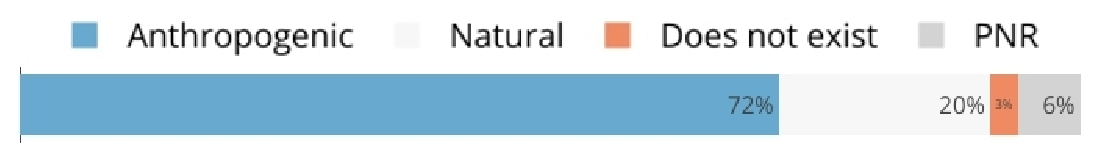
\includegraphics[width=\columnwidth]{Images_EPS/CC_cause_nolegend2.eps}
\caption{Perceived cause of climate change.}
\label{fig:cause}
\end{figure}

\begin{figure}[t]
\centering
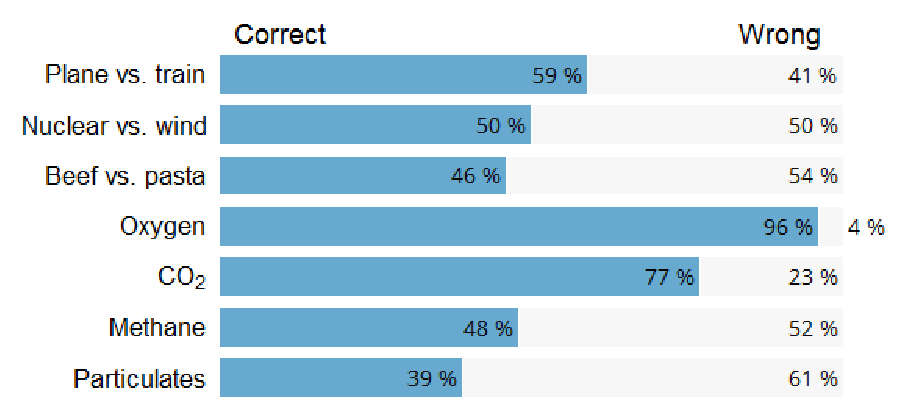
\includegraphics[width=\columnwidth]{Images_EPS/CC_knowledge_valbtr.eps}
\caption{Perceived factors of climate change.}
\label{fig:factors}
\end{figure}

\section{Perceptions and Attitudes over Climate Change\label{sec:attitudes_climate_change}}
    
To fully understand the root motivations to the support or rejection of climate policies, we first analyze the knowledge and perceptions over CC, as well as the reaction that people expect to address this phenomenon. As the paper focuses on explaining attitudes over policies, we relegate to online Appendix 1 some figures and some results from other surveys.
    
    \subsection{Knowledge\label{subsec:knowledge}}
% DONE: cite Sterman 08 -> toujours d'actualité ? => je viens de le relire et oui, c'est consternant de voir à quel point des étudiants du MIT ne comprennent rien. Je le case à côté de Millner & Ollivier
As shown in Figure \ref{fig:cause}, knowledge that CC is anthropogenic is widespread (72\%) and the share who do not believe in climate change (CC) is marginal (4\%). The level of knowledge on the anthropogenic origin of CC is similar to that of other Western countries \citep{leiserowitz_international_2007,lee_predictors_2015,stokes_global_2015-1}: it is 66\% in the U.S. \href{https://news.gallup.com/poll/1615/environment.aspx}{(Gallup, 2019)} for example. At the same time, knowledge about climate science appears limited. Although 77\% of people correctly tick ``CO$_\textnormal{2}$'' as a greenhouse gas (GHG), Figure \ref{fig:factors} shows that almost as many people tick particulate matter (39\%) as methane (48\%). Admittedly, understanding the impacts of activities is more useful than erudition about chemical factors, but here again, knowledge is quite low. We assess such awareness using pairs of comparable activities whose GHG footprint differ by a factor 20 (beef steak vs. pasta, plane vs. train) or whose footprint are similar (nuclear vs. wind power).\footnote{Appendix \ref{app:footprint} details how the figures were obtained.} We ask whether it is true that one activity emits 20 times more GHG than the other, as a way to express precisely that one is ``much more'' polluting than the other. For each pair, around half of the sample is correct. The bulk of respondents pick two correct answers out of three (44\%), but more get them all wrong (19\%) than all right (15\%). 

Not only do most people fail to fully understand the factors and consequences of CC, but they also fail to grasp the degree of reaction needed to tackle it. When informed that ``each French person emits on average the equivalent of 10 tons of CO$_\textnormal{2}$ per year'' and asked what the figure should be in 2050 to ``hope to contain global warming to +2\textdegree{}C in 2100 (if all countries did the same)'', 59\% answer 5 or more (see Figure \ref{fig:target_emission}). Only 17\% select a correct answer: 0, 1 or 2 (see Appendix \ref{app:sources} for why these are correct).

\begin{figure}[t]
\centering
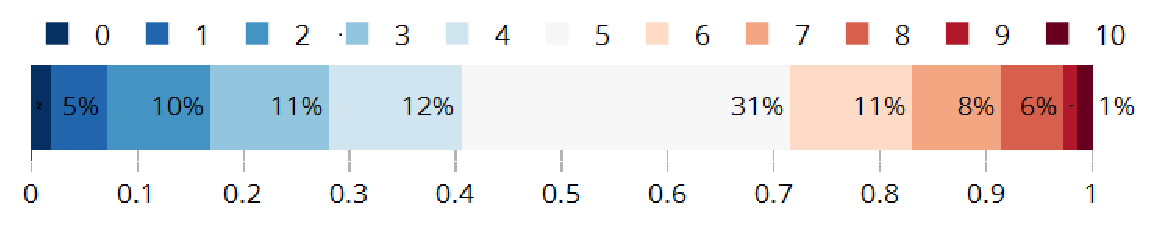
\includegraphics[width=\columnwidth]{Images_EPS/CC_target_emission_nolegend.eps}
\caption{Perceived GHG emission p.c. required in 2050 to limit global warming to +2\textdegree{}C (in tCO$_\textnormal{2}$eq/yr), given that it is now 10.}
\label{fig:target_emission}
\end{figure}

% On pourrait aussi supprimer cette figure du texte principal et la reléguer à l'appendix (pas nécessairement online).


\begin{figure}[!htbp]
\centering
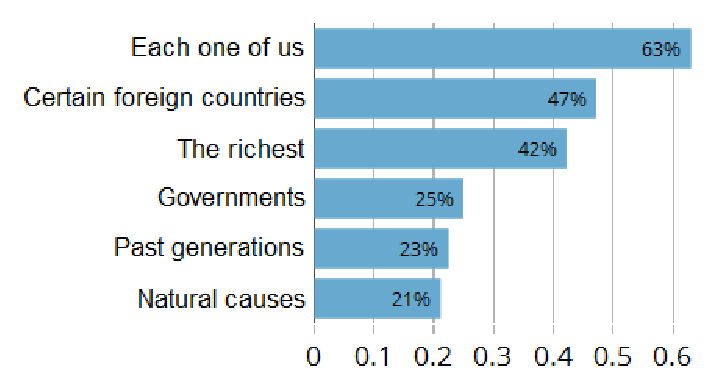
\includegraphics[width=0.75\columnwidth]{Images_EPS/CC_responsiblec.eps}
\caption{Entities perceived responsible for climate change.}
\label{fig:responsible}
\end{figure}

\begin{figure}[t]
\centering
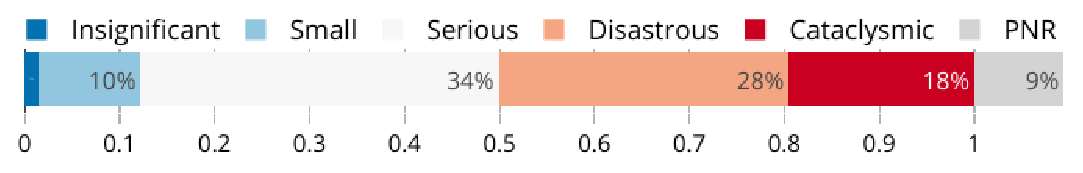
\includegraphics[width=\columnwidth]{Images_EPS/CC_effects_nolegend.eps}
\caption{Perceived gravity of climate change.}
\label{fig:gravity}
\end{figure}

\citet{millner_beliefs_2016} propose several mechanisms to explain people's lack of understanding about climate change: in addition to the difficulty of grasping gradual changes, they emphasize the complexity of drawing a causal link between diffuse causes and distant consequences.\footnote{Actually, even MIT students struggle with this \citep{sterman_risk_2008}.} Failing to assimilate the underlying channels may blur the link between people's own behavior and consequences for the climate. Thus, we can wonder if people understand who would have to make the mitigation effort in a sustainable scenario, i.e. who is responsible for CC.


    \subsection{Positions\label{subsec:opinions}}
    % DONE: Opinions -> Perceptions
% Suggestion!: keep wording after disastrous and grave? 
As shown in Figure \ref{fig:responsible}, 63\% acknowledge that ``each one of us'' is responsible for CC, and less people ascribe the responsibility to ``certain foreign countries'' (47\%), ``the richest'' (42\%), or any other agent.  Not only do people seem lucid concerning the agents causing CC, but a vast majority also foresees worrying consequences if humanity does nothing to limit it. Figure \ref{fig:gravity} shows that 18\% see the impacts as ``cataclysmic, humankind would disappear'', 28\% as ``disastrous, lifestyles would be largely altered'', 34\% as ``grave, because there would be more natural disasters'', while only 11\% think damages would be ``small, because humans would be able to live with it'' or ``insignificant, or even beneficial''. 

% Note: there is also a general tendency to discount one’s own contribution to causing climate change and identify causes of climate change primarily with other people or countries (Lorenzoni & Pidgeon, 2006; Whitmarsh, 2009) (found in Whitmarsh)

% Note: a 1988 survey found that more than three-quarters of respondents were already worried about climate change, rising to almost nine in ten by 1992 (Eurobarometer, 1992). From Whitmarsh 18

Overall, these results indicate that most people understand the fundamentals of climate issues, including the root causes and the scale of the problem, but that only a minority has thought of CC deeply enough to comprehend its factors and the pathways to tackle it.
% Note: cite Kahan 2015 for people understands fundamentals

% parle ~ effets
% inquiétude répandue. Qui est tenu responsable.
    
% autre_op: ADEME 63% conditions de vie extrêmement pénibles en France d'ici 50 ans; 57% pensent pas (probablement ou certainement) que le changement climatique sera limité à des niveaux acceptables d’ici à la fin du siècle (similaire à OpinionWay) / A votre avis qui serait le plus efficace pour résoudre le problème du réchauffement climatique ? 35% chacun d'entre nous, 26% états, 14% instances internationales (aux US c'est plus les entreprises, cf Yale)
% Gallup serious threat to you or your way of life in your lifetime: 45/55

\begin{figure}[t]
\centering
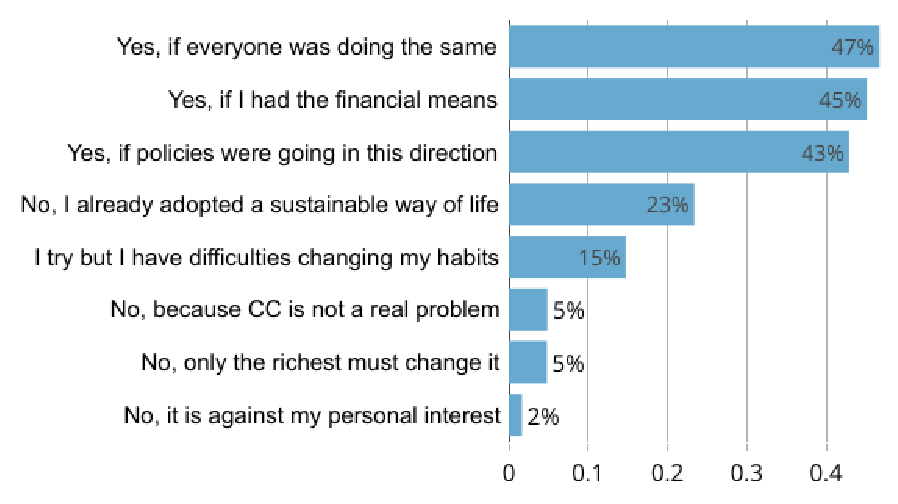
\includegraphics[width=\columnwidth]{Images_EPS/change_if_no.eps}
\caption{Respondent could change their lifestyle under a condition.}
\label{fig:condition}
\end{figure}

    \subsection{The Reaction Needed\label{subsec:reaction}}

Given that many people may not realize the extent of the transition needed to reach sustainability, and that others may be discouraged precisely by the sheer magnitude of such a transition, we can wonder how willing people are to contribute to its success. An encouraging finding for the transition is that 65\% are ``willing to adopt an ecological lifestyle (i.e. eat little red meat and make sure to use almost no gasoline, diesel nor kerosene)'', assuming that ``all states in the world agree to firmly fight climate change, notably through a transition to renewable energy, by making the richest contribute, and imagining that France would expand the supply of non-polluting transport very widely'', while only 17\% answer ``No'' (the others do not take a side). While the phrasing removes most grounds against a change in lifestyle, we inquire under which conditions people would be willing to adopt such a change (see Figure \ref{fig:condition}). 82\% of respondents would be willing to change their lifestyle under at least one of the three conditions proposed: sufficient financial resources, an alignment of policies to this goal, or an adjustment of others' behavior (about 45\% each).
% Done (footnote ajoutée en section 5): définir "warm glow" -> je ne comprends pas trop pourquoi il nous demande de le définir, mais je suggère de remplacer par : "It may be that people overstate their willingness to do good actions, or lack of knowledge regarding the efforts needed, ..." => je ne trouve pas que "overstate" reflète bien le warm glow car on perd le côté "mauvaise foi" (i.e. mensonge à soi-même), et le "willingness" me semble superflu. Pk pas "overstimate their virtue/goodness"? On utilise aussi "warm glow" ailleurs. On pourrait remplacer par "self-deception", "overconfidence" ou "cheap talk" un des deux mais je crois que préfère rajouter une footnote qui explique ce qu'est le warm glow: \footnote{Here, "warm glow" refers to one's unintentional strategy to overestimate their virtue in order to derive satisfaction.} -> Ok, de toute façon cette section va disparaitre du papier. J'ai inséré la footnote à la deuxième mention du terme.

% Pew: 75\% American concerned by CC (Funk Pew 2016)

Finally, a substantial fraction of people incorporates ecological constraints in their life choices. Indeed, 15\% call themselves ecologist (the most picked political identity outside of the left-right spectrum, see Appendix \ref{app:stats_des}), 23\% claim they already adopted a sustainable way of life, and 20\% say the CC ``has had or will have an influence in their decision to have a child''. 

% Cited from Kallbekken and Aasen (2010) : "a poll of 22,000 respondents from 21 countries found that 83% say it will be necessary to make lifestyle and behavioural changes to reduce emissions of greenhouse gases (Globescan and PIPA, 2007)."

% autre_reaction: ADEME  Si des changements importants s’avèrent nécessaires dans nos modes de vie, à quelles conditions les accepteriez-vous ? 45% qu'ils soient partagés de façon juste entre tous les membres de notre société, 11% Qu'ils restent dans des proportions modérées, je ne suis pas prêt à accepter des changements radicaux dans mon mode de vie, 15% accepterai dans tous cas / fait déjà: moins viande 45%, vélo/pied plutôt que voiture 35%, consommer moins 47% ; peut pas-difficilement moins voiture : 16-19% (plus optimiste qu'IFOP 11, cf. aussi OpinionWay), 8-15 viande
% OpinionWay: aliments de saison, local, "réduire conso, recycler, échanger", plus de marche et vélo sont les efforts personnellement prêts à être consentits par une majorité, privilégier transports en commun 34%, le train ou le bus à l'avion pour longues distances 21%, "consommer moins de viande, d'oeufs et de produits laitiers" 31%
% BVA 58% pensent qu'ils consommeront moins d'énergie dans 10 ans en 2011, 61% veulent faire réaliser des travaux d'économie d'énergie et 76% changer leurs habitudes de consommation, 48% pensent utiliser le solaire dans les 20 prochaines années 
% Gallup 52% think they do a good job at protecting env


\section{Attitudes over Carbon Tax and Dividend} \label{sec:attitudes_carbon_tax}

%Objective of this section: in the companion paper we show that people reject the tax because they are biased. We focused on three critical determinants. Beyond these motives, we want to understand more how people perceive the carbon tax, and what makes them reject it.

%In our companion paper we assess respondents beliefs over the tax properties, in particular over their self-interest, the tax's effectiveness and progressivity. 

% DONE:  our survey presents to respondents -> we investigate the preferences over
Most French people are aware and concerned about climate change and claim to be willing to exert efforts to fight it. Yet, the government's attempt to introduce a carbon tax to deal with French emissions resulted in a widespread popular protest. To understand this paradox, we investigate the preferences over a Tax \& Dividend policy: an increase of 50\euro{}/tCO$_2$ in the current French carbon tax, with a uniform lump-sum redistribution of the additional revenue to all adults. This policy differs from the official one whose revenue was mostly used to fund the general budget. Respondents are given the associated increase in energy prices so that the direct costs are salient: $+13\%$ (resp. $+15\%$) for gas (resp. domestic fuel), and $+0.11$\euro{} (resp. $+0.13$\euro{}) for a liter of gasoline (resp. diesel). They are also told that the transfer would amount to 110\euro{} per adult annually. %In this section we examine people's perception about the policy, in particular the associated problems and benefits, as well as the category of people who would win or lose according to them.

    \subsection{Widespread rejection}

% dire que les gens sont biaisés et renvoyer vers l'autre papier. 
French people would largely reject the proposed policy. Only 10\% of our respondents declare they would approve it, while 70\% say they would not (see Figure \ref{fig:approval}). As shown in our companion paper \citep{douenne_can_2019}, this rejection can be explained by erroneous perceptions about the policy's outcome, such as an overestimation of its impact on one's purchasing power. For instance, 30\% of people who use neither gas nor domestic fuel believe their household would lose from an equally redistributed increase in taxes on these goods. Interestingly, the salience of costs appears critical in people's answer. At a later stage of the survey, we ask respondents whether they would agree to increase the carbon tax if the revenue was returned to all households, without mentioning the impact on prices. The question is asked along with a package of other environmental policies (see section \ref{sec:attitudes_other_policies}). In this case --- where the benefits are more salient than the costs --- we find a much higher approval rate of 37\%. Another survey conducted in March 2019 (\href{https://drive.google.com/file/d/1ne1nUsJJqY1PYFOs9dH9uK6mLw39R1QY/view}{OpinionWay, 2019}) assesses acceptance for a \textit{reintroduction} of the carbon tax increase in 2021. They find intermediary results with an approval rate of 21\%. % 21\% of people approving it vs. 77\% opposing it.

% Suggestion: La phrase avec 30\% n'est pas nécessaire ici, pourrait être supprimée

\begin{figure}[t]
\centering
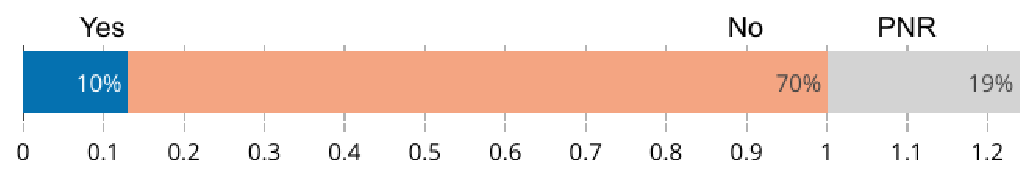
\includegraphics[width=\columnwidth]{Images_EPS/approval_trim.eps}
\caption{Approval of Tax \& Dividend.}
\label{fig:approval}
\end{figure}
%French people would largely reject the proposed policy. Only 10\% of our respondents declare they would approve it, while 70\% say they would not (see Figure \ref{fig:approval}). As shown in our companion paper \citep{douenne_can_2019}, this massive rejection can be explained by erroneous perception about the policy's outcome, such as an overestimation of its impact on one's purchasing power. Another survey (\href{http://www.datapressepremium.com/rmdiff/2008572/Etude-OpinionWay-pour-PrimesEnergie.fr.pdf}{OpinionWay, 2019}) has also assessed acceptance for a carbon tax. Their phrasing differs from ours as they do not make the policy costs salient nor specify the rate of the tax increase and the use of the revenue. They still found comparable results, with 21\% of people approving an increase of the tax in 2020, and 77\% opposing it (2\% ``PNR''). At a later stage of the survey, we also ask whether people would agree to increase the carbon tax if the revenue would be returned to all households, without expliciting the price increase. In this case, where the benefits are more salient than the costs, we also find a higher approval rate of 37\%.

% Note: attention plusieurs sondages opinionway en mars 2019

The low level of acceptance observed partly results from recent events. In July 2018, \citet{ademe_representations_2018} found that 48\% of French people thought it was desirable to increase the carbon tax, a figure similar to those of other countries \citep{brechin_public_2010}. The discrepancy between 2018 and 2019 can be explained by the ``campaign effect'' highlighted by \citet{anderson_can_2019}: support for a carbon tax decreases substantially after it enters the public debate. Indeed, the French carbon tax was brought under the spotlight in the end of 2018, after high oil prices triggered the Yellow Vests movement.
%At that time, the carbon tax had been in place for more than four years, but low oil prices made its existence little known. A few months later, in a context of higher barrel prices, the tax was put under the spotlight and its associated costs became more salient, fostering the strong opposition.
% Suggestion: cite Carattini, Kallbekken, and Orlov (Nature 2019)
% Yale p. 16 show evidence that it is influenced by salience of costs, as 61% support a carbon tax on fossil fuel companies whose revenues would pay down the national debt, but 39/66 support increase by 0.25$/gallon to reduce federal income tax or 38/56 if it costs $180/year per household or 43/26 if tax refund given to every household. -> Les deux politiques diffèrent trop pour que l'on puisse réduire la différence de soutien à la saillance des coûts.

% Done : (" thought is was desirable" -> " thought it was desirable")

% Suggestions sondages

%  « La mise en place d’une taxe sur la consommation d’énergie non renouvelable (pétrole, gaz, fioul, charbon…) et sur les émissions de gaz à effet de serre» : 11/33/38/18 ; « souhaitez-vous qu'une taxe carbone soit mise en place à l'échelle de l'Union Européenne ? » : 23/39/15/18 ; « Le gouvernement envisage d’instaurer pour les particuliers et les entreprises une contribution « climat-énergie » ou taxe carbone sur les énergies polluantes comme le gaz, le pétrole ou le fioul. Personnellement, seriez-vous tout à fait, plutôt, plutôt pas ou pas du tout favorable à cette mesure ? » : 6/28/23/42 (2009 : les gens ont changé ou c'est l'effet montré par la pote d'E. Guillaud, à savoir que les gens sont d'accord jusqu'à ce que ça les impacte vraiment ?)
% fiscalité 57% contre la mise en place d'une fiscalité écologique BVA 2013

% autre_tax: ADEME 55% pour augmenter la taxe carbone 
% DYNEGAL: 56% pour une taxe sur les émissions de gaz à effet de serre selon le principe pollueur = payeur / 49% contre les taxes pour décourager certains comportement (50/50) mais 77% pour quand il s'agit de réductions d'impôt / 6/38/29/24% tout à fait à pas du tout prêt à payer plus d'impôts pour protéger l'environnement
% 56% contre rétablissement taxe carbone 4/04/19 https://www.lejdd.fr/Politique/sondage-tva-redevance-audiovisuelle-les-francais-plebiscitent-les-suppressions-de-taxes-3887510

    \subsection{Perceived winners and losers}

Figure \ref{fig:winners_losers} represents the share of respondents who expect different household categories to win or lose from the policy. Income appears to be the most critical divide, with a non-monotonic relationship. 30\% of respondents expect the richest to win while only 2\% think they would lose. On the contrary, 40\% more people think that the poorest would lose rather than win, a difference even higher for the middle class --- the category most expected to lose --- at 53\%. To half of respondents, we framed the question about winners and losers specifically in terms of ``purchasing power''. The objective was to see if some categories were commonly seen as losing in welfare although they could gain in monetary terms, or conversely. The results look very much alike for both formulations, except that the shares of people expecting poorer households to gain (5.8\%) and richer households to lose (0.9\%) are significantly larger when asked in terms of purchasing power: 10.2\% and 2.1\%, respectively (see online Appendix 2). Overall, respondents perceive the Tax \& Dividend as regressive. As shown by a large body of literature \citep[e.g.][]{west_williams_04,bento_distributional_2009,williams_initial_2015}, and more specifically in our companion paper \citep{douenne_can_2019}, these beliefs are at odds with the true distributive effects of this proposed policy. % since poorer households net gains exceed on average those of richer households.
% : 5.8\% of people expect poor households to win, but 10.2\% expect them to win in monetary terms. Conversely, only 0.9\% expect rich households to lose, but 2.1\% to lose financially.
\begin{figure}[t]
\centering
\begin{subfigure}[b]{\columnwidth}
   \caption{Winners}
   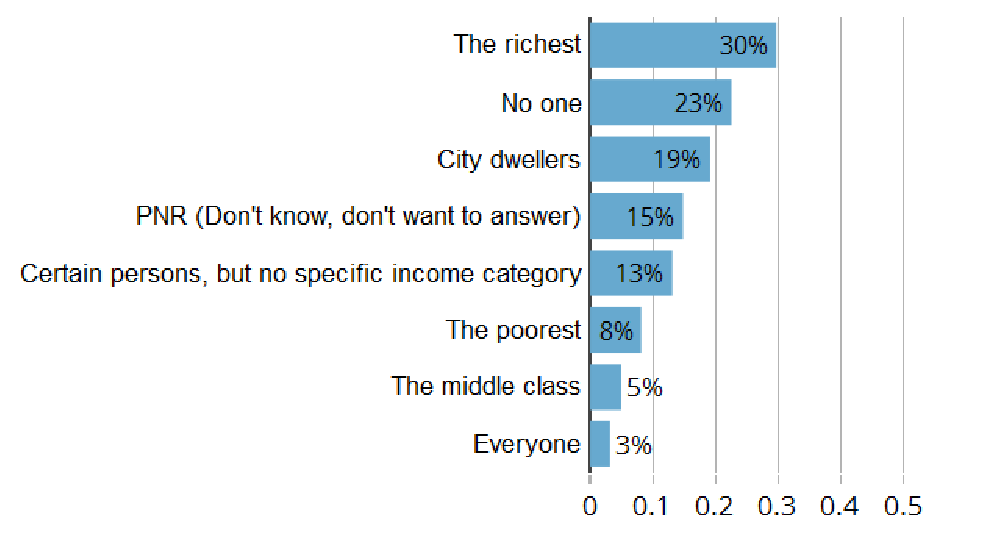
\includegraphics[width=\columnwidth]{Images_EPS/tax_winners_synchro.eps}
\end{subfigure}

\begin{subfigure}[b]{\columnwidth}
\vspace{0.3cm}
   \caption{Losers}
   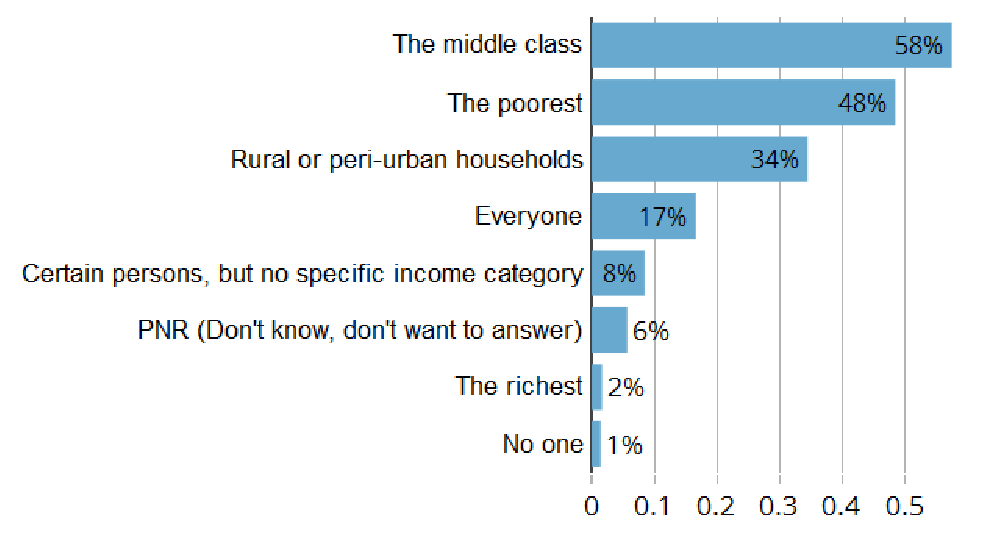
\includegraphics[width=\columnwidth]{Images_EPS/tax_losers_synchro.eps}
\end{subfigure}
\caption{Perceived winners and losers from Tax \& Dividend}
\label{fig:winners_losers}
\end{figure}

Beyond the income dimension, people tend to identify city dwellers as potential winners from the Tax \& Dividend (third position at 19\%), while rural and peri-urban households are rather expected to lose (third position at 34\%). We also see that people report on average more categories for expected losers than winners: 1.74 vs. 1.16. The high ranks of ``no one'' for winners (second) and of ``everyone'' for losers (fourth) further suggest that respondents do not see our policy as a zero-sum game. % unclear that no/every one are excluded. But it doesn't matter as the shares are comparable for no one and everyone (23 vs 17%)
% , with respectively 1.74 and 1.16 categories selected on average
    \subsection{Perceived pros and cons}

% dire que la taxe envisagée réduirait les émissions de façon marginale -> on le dit plus bas, à voir si on le déplace ici

% This belief that the tax would be ineffective is shared by 66\% of respondents, while only 17\% do think it would be effective (18\% ``PNR''). -> on pourrait éventuellement le mettre en footnote.

Previous studies have highlighted that distributive effects are a critical determinant of carbon tax acceptance \citep[e.g.][]{kallbekken_saelen_2011,brannlund_tax_2012,gevrek_public_2015}. When asked about the problems associated with the Tax \& Dividend, the main response is that the tax would penalize rural households (47\%). Interestingly, this concern comes before the threat that the tax could penalize the poorest (sixth position with 29\%), although more people report the poorest as a category of people expected to lose. The second and third concerns are that the policy is simply a pretext to increase taxes (43\%) --- a worry documented by \citet{dresner_social_2006} and \citet{klok_et_al_2006} --- and that it would be ineffective to reduce pollution (37\%). Related to this last point is the perceived lack of alternatives, seen as insufficient or too expensive (31\%). This problem has been previously stressed by \citet{kallbekken_aasen_2010} in a focus group study: people do not see the point of taxing fossil fuels if they cannot substitute for other technologies. This last reason is stated as frequently as concerns over the impact on one's own purchasing power (fourth with 31\%). As shown in \citet{douenne_can_2019}, self-interest largely affects acceptance of the Tax \& Dividend, but this concern could sound too egoistic when stated in a direct way. While previous studies have pointed out concerns over the negative impact of carbon taxation on the economy \citep[e.g.][]{thalmann_public_2004,carattini_green_2017}, this problem comes last (14\%) and does not seem to represent an important obstacle for public support in the current context. % instead of "France", parce que des auteurs montrent que le soutien varie avec la conjoncture -> Ok oui ça aurait peut-être été différent il y a quelques années

% The second and third concerns are that the policy is just a pretext to increase taxes (43\%) --- a worry documented by \citet{dresner_social_2006} and \citet{klok_et_al_2006} --- and would be ineffective to reduce pollution (37\%). These two reasons are stated more frequently than concerns over the impact on one's own purchasing power (fourth with 31\%). As shown in \citet{douenne_can_2019} self-interest largely affects people acceptance of Tax \& Dividend, but this concern could sound somewhat egoistic when stated in a direct way. A last important perceived problem is the lack of alternatives, seen as insufficient or too expensive (31\%). This problem had been previously stressed by \citet{kallbekken_aasen_2010} in their focus group study, and is intrinsically linked to beliefs of ineffectiveness.

\begin{figure}[t]
\centering
\begin{subfigure}[b]{\columnwidth}
   \caption{Benefits}
   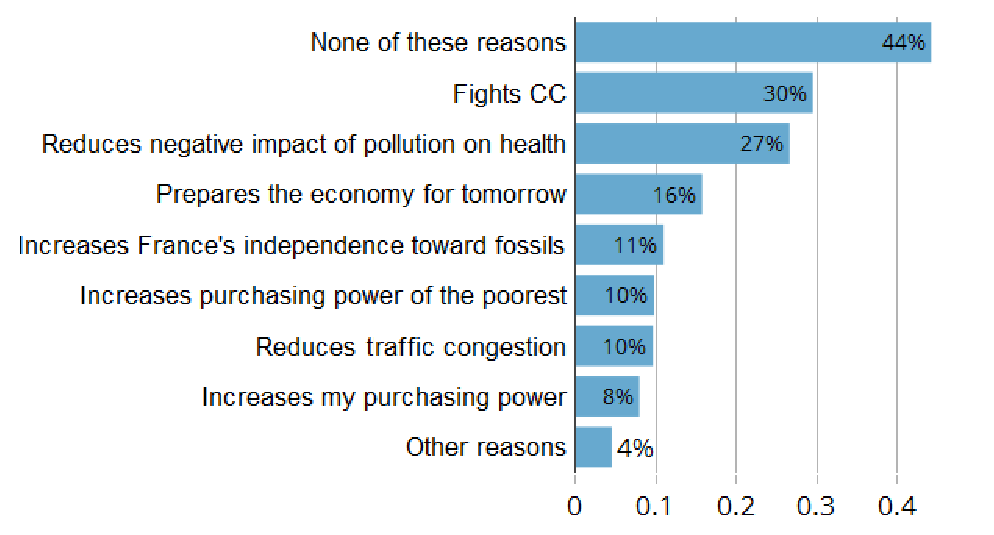
\includegraphics[width=\columnwidth]{Images_EPS/CC_benefits_synchro.eps}
\end{subfigure}

\begin{subfigure}[b]{\columnwidth}
\vspace{0.3cm}
   \caption{Problems}
   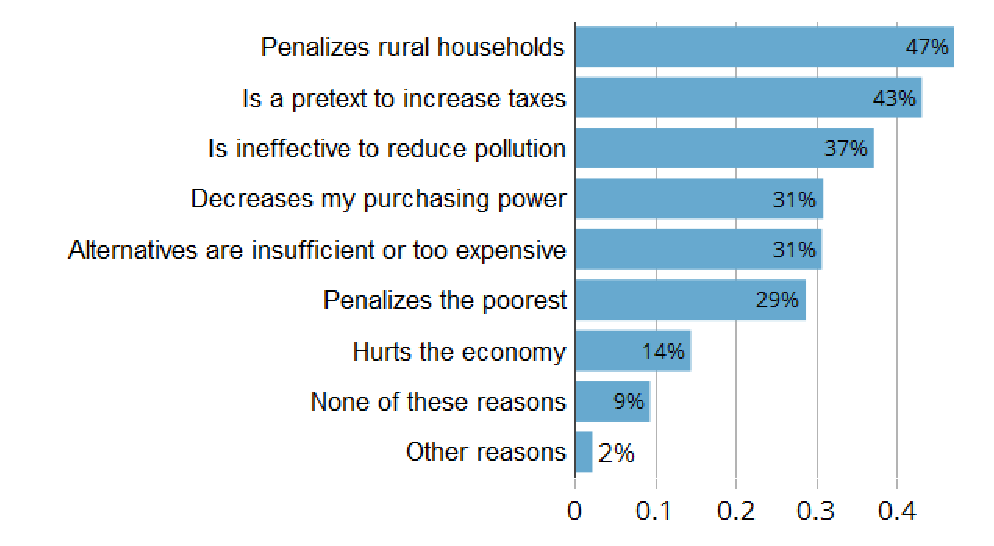
\includegraphics[width=\columnwidth]{Images_EPS/CC_problems_synchro.eps}
\end{subfigure}
\caption{Perceived benefits and problems from Tax \& Dividend}
   \label{fig:benefits_problems}
\end{figure}

Respondents are suggested to pick at most three answers among both problems and benefits. On average, respondents pick 2.36 problems --- and 53\% pick at least 3 --- against 1.14 benefits, excluding the most popular: ``None of these reasons'' (44\%). This option comes far ahead of the second and third, ``fight climate change'' (30\%) and ``reduces negative impact of pollution on health'' (27\%). Still, environmental benefits are much more cited than economic ones. This result is likely due to people's pessimism about the outcome of the policy, but it might also reflect the limited importance given to economic consequences of the carbon tax, as already suggested by problems commonly cited. %  --- if only a few actually anticipate economic benefits --- 
% Murray & Rivers (2015) showed increased support overtime in British Columbia (reject before implementation, support afterwards)

    \subsection{Consumption and mobility constraints}

The perceived problems identified above suggest a rationale for people's opposition towards carbon taxation: if people think the tax is ineffective, because their consumption is constrained and affordable alternatives are lacking, then taxing carbon can be perceived as a pretext to increase taxes. % narrative

    \subsubsection{Perceived elasticities}

In order to understand to what extent people feel constrained with respect to their energy consumption, we elicit their subjective price elasticity for transport and domestic energies. We adopt the phrasing of \citet{baranzini_effectiveness_2017} and ask the expected decrease in energy consumption that would follow an increase in prices. To avoid dealing with small percentages, which people usually find more difficult to compare, we ask for the reaction to a 30\% increase in the price of heating (or equivalently, an increase of 0.50\euro{} per liter in fuel prices). Although sufficiently high to foster a significant response on demand, these changes are realistic in the medium run, and should not lead people to report long-term elasticities. Respondents may select their answer among 5 brackets. They are asked to estimate their own reaction as well as that of French people. Figure \ref{fig:elasticities_agg} presents the results.

% DONE: supprimer ici aussi le "To do so," ?

\begin{figure}[t]
\centering
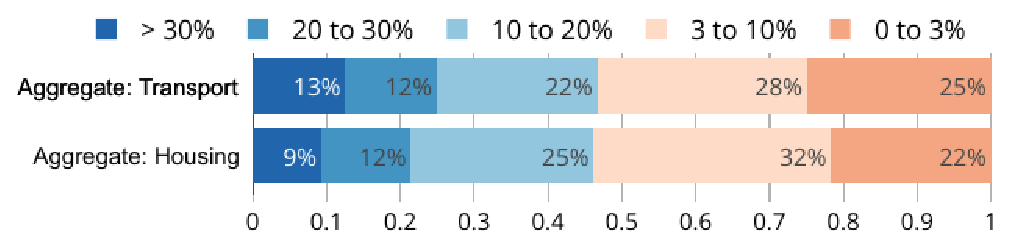
\includegraphics[width=\columnwidth]{Images_EPS/elasticities_agg_valb.eps}

\includegraphics[height=0.3cm]{Images_EPS/blank.eps}
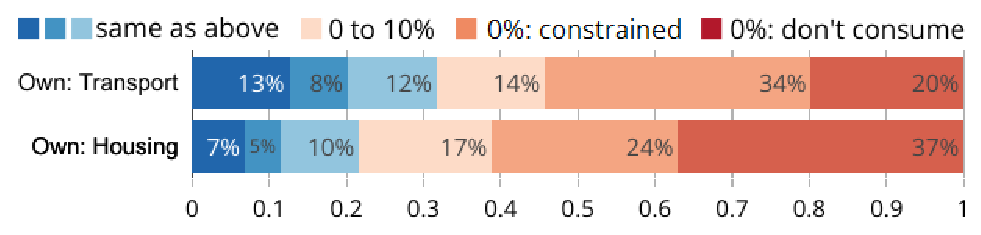
\includegraphics[width=\columnwidth]{Images_EPS/elasticities_perso_valbuena.eps}
\caption{Perceived aggregate and own elasticities.}
\label{fig:elasticities_agg}
\end{figure}

\begin{figure}[b]
\centering
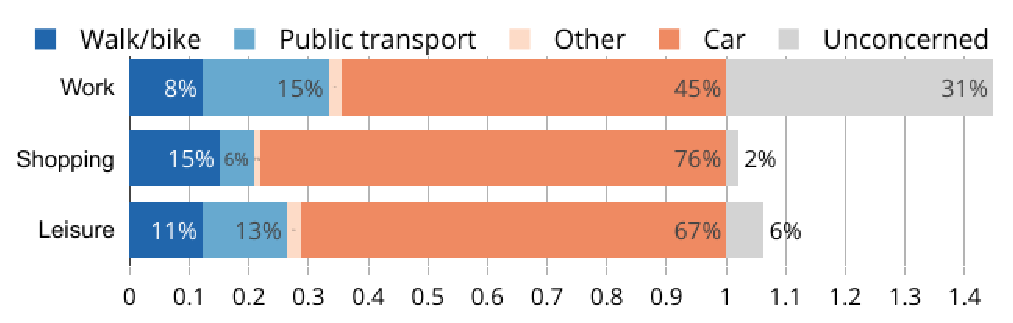
\includegraphics[width=\columnwidth]{Images_EPS/transports_use_trim.eps}
\caption{Mode of transportation by activity.}
\label{fig:transports_use}
\end{figure}

% Suggestion: "in both cases" 40\% of people expect...: give stat for fuel? -> the stat works for both: 34/(100-20)=42.5, 24/(100-37)=38
54\% (resp. 61\%) of respondents consider that such an increase in prices would not lead them to reduce their transport (resp. domestic) energy consumption. This expected inelastic behavior is mainly due to mobility constraints for transport (64\% of cases) while it mostly reflects a non-fossil heating type for housing (61\%). Excluding people reporting inelastic behavior because of insignificant initial consumption, about 40\% of people feel constrained and expect to not lower their consumption following price increases. Still, respondents perceive transport fuel price elasticity of French people at $-0.45$ on average, and their own elasticity at a consistent $-0.36$ (after re-weighting by fuel expenditures). Concerning housing energy, aggregate and personal subjective elasticities are respectively $-0.43$ and $-0.33$. Overall, these subjective elasticities compare well to the ones found in the literature for French households, although they are slightly over-estimated (in absolute value) for housing.\footnote{For transports, estimates from the literature lie around $-$0.4 \citep{clerc_marcus,bureau_distributional_2011,douenne_vertical_2018}. For housing, the values are lower, typically around $-$0.2 \citep{douenne_vertical_2018,clerc_marcus}.}

% Old : Overall, these subjective elasticities compare well to the ones found in the literature for French households: around $-$0.45 for transport fuels \citep{clerc_marcus,bureau_distributional_2011,douenne_vertical_2018} and $-$0.2 for housing \citep{douenne_vertical_2018,clerc_marcus}.

%\citet{douenne_vertical_2018} found very close estimates for the uncompensated price elasticity of transport fuels, at $-$0.45, in the typical range of the literature \citep[e.g.][]{clerc_marcus,bureau_distributional_2011}. For housing energies, the subjective values reported tend to exceed common estimates that rather lie around $-$0.2 \citep{douenne_vertical_2018,clerc_marcus}. This result is possibly due to the lack of salience of domestic energy prices and the hassle to replace equipment, hence the low actual response in the short-run to variation in prices despite people's intended reaction.

% Note: 45\% of respondents see themselves as strictly more constrained than average for fuel consumption, which is close with the objective share of households who spend more fuel than average: 41\%. Correlation of 0.22 between . 

% Suggestion: 50% correlation between own and aggregate elasticities, suggesting that people understands well their own reaction but wrongly project it on the whole population.

% Note: on other countries, see the meta-analysis of Brons et al (2008) "A meta-analysis of the price elasticity of gasoline demand. A SUR approach" for gasoline. For electricity (not all residential energies), see Espey and Espey (2004).

\begin{figure}[t]
\centering
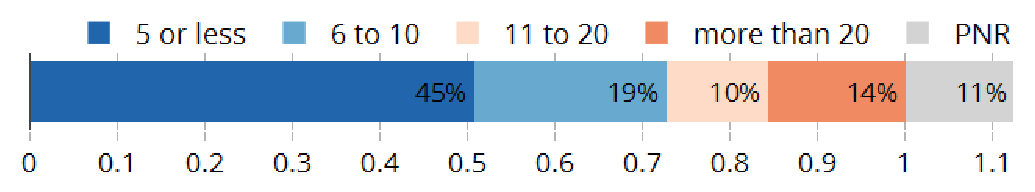
\includegraphics[width=\columnwidth]{Images_EPS/transports_distance_trim.eps}
\caption{Walking distance to the nearest stop, in minutes.}
\label{fig:transports_distance}
\end{figure}

\begin{figure}[t]
\centering
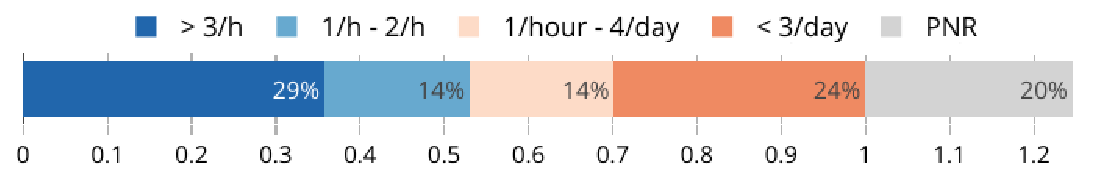
\includegraphics[width=\columnwidth]{Images_EPS/transports_frequency_trim.eps}
\caption{Frequency of public transport at the nearest stop.}
\label{fig:transports_frequency}
\end{figure}

\begin{figure}[b]
\centering
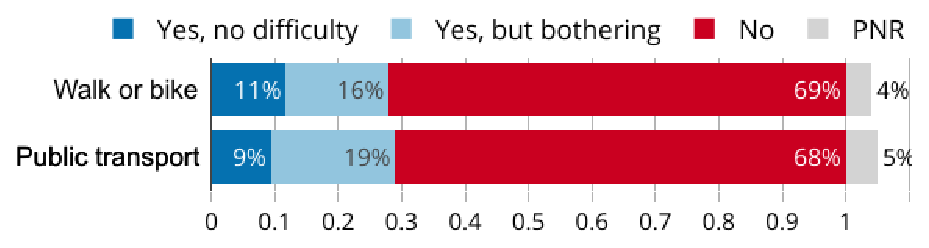
\includegraphics[width=\columnwidth]{Images_EPS/transports_work.eps}
\caption{Among those who commute to work by car, possibility to change the transportation mode, depending on the alternative.}
\label{fig:transports_work}
\end{figure}
    
\begin{figure}[b]
\centering
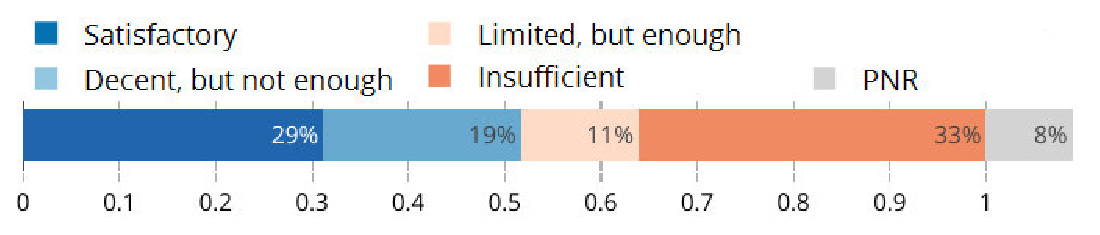
\includegraphics[width=\columnwidth]{Images_EPS/transports_opinion_trim.eps}
\caption{Supply of public transport where the respondent lives.}
\label{fig:transports_opinion}
\end{figure}

    \subsubsection{Mobility and public transport}
    % Suggestion: références dans le doc.

To assess the level of dependence on automobiles, which we include as a determinant for preferences in Section \ref{sec:determinants}, we study mobility habits and access to public transport. Figure \ref{fig:transports_use} indicates that 65\% of employed people drive to work, and that car usage is even more common for grocery shopping or leisure activities. This figure is confirmed by the national transport survey \href{http://www.progedo-adisp.fr/enquetes/XML/lil-0634.xml}{ENTD (2008)} conducted by Insee and analyzed in \cite{pappalardo_mobilite_2010}, which reveals that a majority still uses a car for trips of 1 to 2 km. Even though 73\% live within a 10 minute walk to a public transit stop (Figure \ref{fig:transports_distance}), coverage and frequency of public transport is often too low (Figure \ref{fig:transports_frequency}) to compete with the speed, comfort, and flexibility of automobiles. Indeed, 58\% of those who commute by car declare that they could neither substitute it with public transport nor walking or cycling, and only 15\% could use one of these alternative without major difficulties (Figure \ref{fig:transports_work}). Further evidence indicates that the lack of alternatives is a main factor for car usage, besides apparent taste for a vehicle that remains a symbol of freedom. Figure \ref{fig:transports_opinion} shows that 52\% of respondents state that supply of public transport where they live is ``insufficient'' or ``decent, but should be increased'', while 40\% find it ``satisfactory'' or ``limited, but sufficient''. From this perspective, ``green public investments and carbon taxes appear to be complementary, and in the timing of climate policy it would be justified to carry out the former before implementing the latter'', as \cite{bureau_pour_2019} suggest. Alongside an increase in the supply of alternatives, climate policies could also address the demand for mobility, e.g. by revitalizing town centers and limiting urban sprawl.

% Our answers mix objective and subjective characterisation of public transport supply to account for the variation in expectations for the supply depending on the density of an area. On the objective side as well, nearly half of people with an opinion find the supply ``limited'' or ``insufficient'' (48\%). 

% Suggestion: some figures conditional on rural/peri-urban areas

%" Dans cette optique, investissements publics verts et taxe carbone apparaissent bien complémentaires, et dans le timing de la politique climatique il serait justifié de réaliser les premiers avant de mettre en place la seconde" note CAE
% "La tendance structurelle à l’étalement urbain doit être infléchie pour réduire les émissions du secteur des transports, ce qui requiert des villes accessibles financièrement et attrayantes." note CAE
% ADEME vélo/pied plutôt que voiture 35%

% Même si les trois quarts des Français vivent à moins de 15 minutes de marche d'un arrêt de transports en commun, la Table \ref{tab:transports} montre qu'une majorité d'entre eux juge l'offre de transports en commun insuffisante, en particulier en zone rurale et dans les petites villes. Sur les 65\% de répondants qui se rendent en voiture à leur travail, 58\% affirment ne pas pouvoir s'y rendre en transports en commun, à pied ou à vélo, et seuls 15\% pourrait utiliser un de ces modes de transport alternatif ``sans grande difficulté''. Le caractère incontournable de la voiture individuelle semble être une limite majeure aux mesures purement incitatives, même si celles-ci sont nécessaires pour bousculer les habitudes, alors que \href{https://www.alternatives-economiques.fr/part-differents-modes-de-transport-fonction-de-distance-domicile-travail-effectuee-actifs-ayant-un-0112201781570.html}{62\% des trajets de 1 ou 2 km sont effectués en voiture}. 

\section{Attitudes over Other Policies}\label{sec:attitudes_other_policies}

The previous section has shown that our Tax \& Dividend was largely rejected by French people. As climate policies are urgently needed, it appears necessary to assess whether other designs and instruments would be met with a higher support. This section first examines public opinion about several alternative uses for the carbon tax revenue and then turns to other environmental and climate policies.

    \subsection{Preferred Revenue Recycling}
% cite Beiser & Bernauer 2019

%A large body of literature has shown that people tend to see Pigouvian taxes as ineffective to reduce pollution \citep[e.g.][]{dresner_social_2006,kallbekken_et_al_2011, baranzini_effectiveness_2017}. Our companion paper confirms this result, shows that people also wrongly see Tax \& Dividend as regressive, and overestimate its impact on their own purchasing power. As we these biases have been shown detrimental for acceptance, we can wonder whether other uses of the revenue would lead to similar opposition. To answer this question, w
We asked respondents to what extent they would accept an increase in the carbon tax for different uses of the revenue. As the exact cost of the tax was not specified, the benefits of the revenue recycling were made relatively more salient, which explains higher acceptance rates compared to our Tax \& Dividend. Still, this question enables to compare answers relative to one another.

        \subsubsection{Investments in energy transition}

%people who would approve raising the carbon tax in this case
%a large body of literature
% The financing of non polluting transports comes first with 65\% of approval. Investments in renewable energies and thermal renovation of buildings come third and fourth with approval rates of respectively 59\% and 56\%. 
Figure \ref{fig:recycling} reports people's responses to each proposed scenario. Overall, the preferred revenue recyclings are investments in the energy transition. This result is consistent with various papers showing that earmarking the revenue of the tax for environmental purposes largely increases public support \citep[for a review of the literature, see for instance][]{kallbekken_aasen_2010,carattini_overcoming_2018}. As people tend to see carbon taxation as effective only if it finances green investments \citep{saelen_kallbekken_2011}, these policies legitimize the implementation of a tax and increase its acceptance. In addition, the large approval for a policy investing in non-polluting transport can be explained by people's desire for mobility alternatives, the lack of which was identified as an important problem with our Tax \& Dividend (see section \ref{sec:attitudes_carbon_tax}). % DONE: mechanisms -> policies

% Old: The large approbation for a policy investing in non-polluting transports can also be explained by people's will for mobility alternatives. Among the 31\% of households who selected the lack of alternatives as a problem of Tax \& Dividend (see section \ref{sec:attitudes_carbon_tax}), the approval rate for a carbon tax invested in non polluting transports goes up from 65\% to 71\%, with only 13\% disapproving.

% \href{http://www.odoxa.fr/sondage/baro-eco-francais-jugent-desormais-compatibles-defense-de-lenvironnement-politiques-economiques-favorisant-croissance-lemploi/}{Odoxa 2019} on thermal renovation (86\%), electric car subsidies (65\%) or carbon tax (20\%)

\begin{figure}[!htbp]
\centering
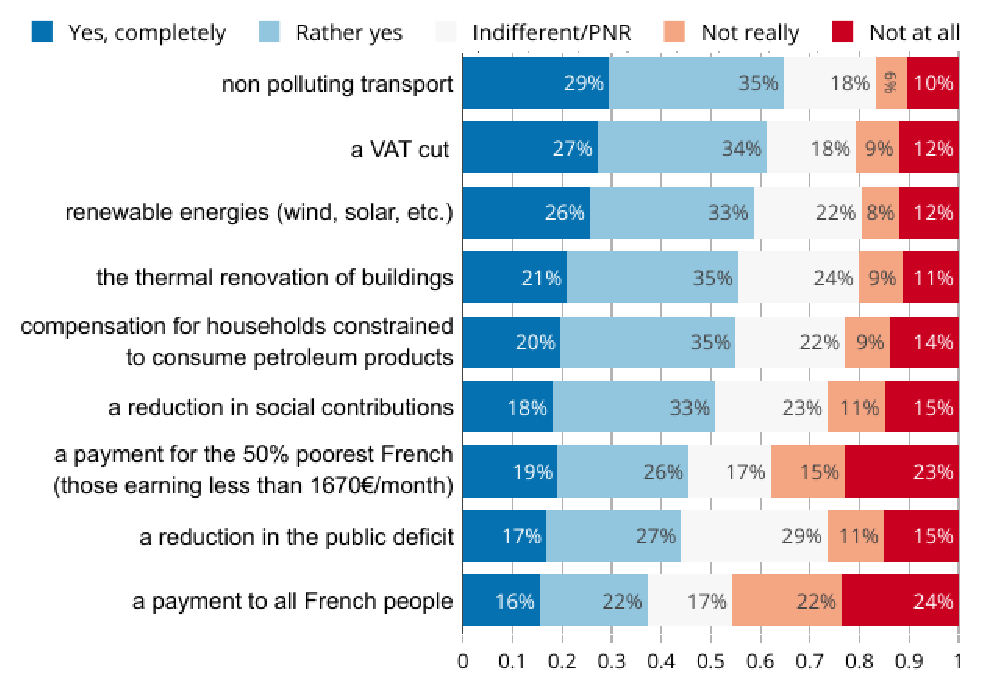
\includegraphics[width=\columnwidth]{Images_EPS/tax_condition_valc.eps}
\caption{Approval of a carbon tax if its revenue finances...}
\label{fig:recycling}
\end{figure}

        \subsubsection{Transfers to households}
% As discussed in section \ref{sec:attitudes_carbon_tax}, the approval rate (37\%) still exceeds the one initially obtained for our Tax \& Dividend policy, since the emphasis in this question is on the transfer and the costs are not salient. When targeted to the bottom 50\% of the income distribution, these transfers are slightly more approved (46\%) although this alternative ranks only seventh out of nine.
While previous literature has shown that distributive concerns matter for carbon tax approval, the common tool proposed by economists to address this issue --- lump-sum transfers --- is not met with resounding support. Out of the nine proposed mechanisms, the standard flat recycling comes last (with 37\% approval), and a transfer targeted to the bottom 50\% comes seventh (46\%). Consistent with our previous finding that people are concerned that the carbon tax may penalize rural and peri-urban households, the preferred ``lump-sum'' transfer is the one targeted to people constrained with respect to their consumption of petroleum products (fifth with 55\% approval). These results echo the findings of \citet{kallbekken_et_al_2011} who showed that people tend to prefer more narrowly targeted revenue recycling, possibly because of distributional concerns. The lower support for transfers is the only result that departs from the preferred revenue recycling in Germany and in the U.S., documented by \citet{beiser-mcgrath_could_2019}.% DONEw

The relatively low support for compensation mechanisms should however not be understood as a lack of concern about purchasing power or distributive effects. As shown in section \ref{sec:attitudes_carbon_tax}, the distributive properties of lump-sum transfers are not well understood. Perhaps surprisingly, the second preferred mechanism for revenue recycling is a reduction in the VAT rate (61\% approval). The main rationales for this support are the benefits to one's purchasing power and the perceived distributive effects. As the VAT is known to be a regressive tax, people may perceive it fair to compensate an increase in the regressive carbon tax with a decrease in the VAT. Although such a mechanism would be less favorable to poorer households --- who spend less in VAT in absolute value, and would therefore receive less than from a uniform transfer --- it may not be perceived as such. % and therefore chosen over lump-sum transfers.

% Thalmann sur TVA vs. taxe carbone ? -> on le cite déjà beaucoup

        \subsubsection{Double dividend and public deficit}

The last two options propose to use the carbon tax revenue to reduce social contributions, or the public deficit. These mechanisms come respectively in sixth and eighth position with 51\% and 44\% of approval. These results can be linked to the low level of concern regarding the impact of a carbon tax on the economy documented in section \ref{sec:attitudes_carbon_tax}. They are also consistent with previous focus group studies \citep[e.g.][]{kallbekken_aasen_2010}, including in France where \citet{deroubaix_rise_2006} found that people did not understand why the revenue of an environmental tax reform should be used to tackle unemployment.


\begin{figure}[t]
\centering
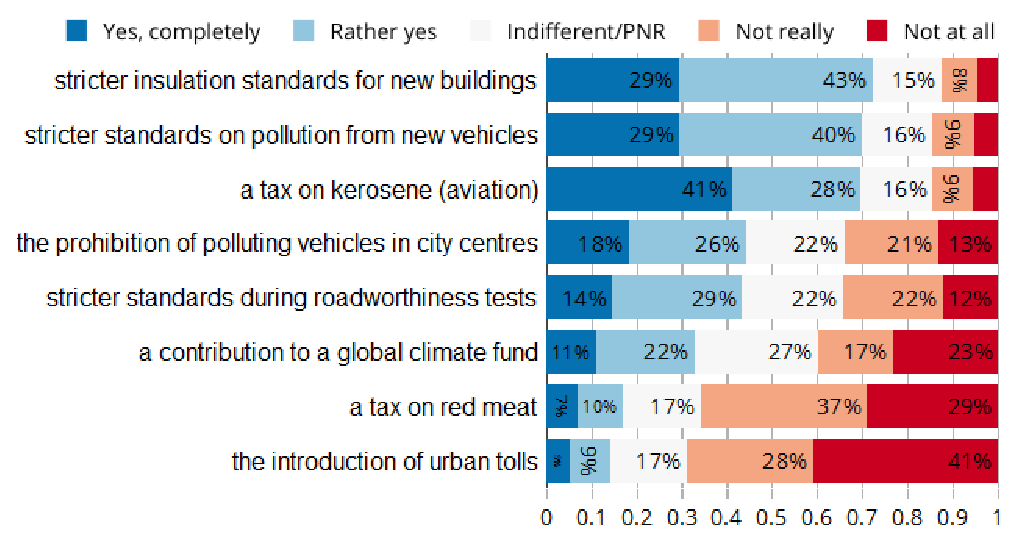
\includegraphics[width=\columnwidth]{Images_EPS/environmental_policies.eps}
\caption{Approval of different climate policies.}
\label{fig:policies}
\end{figure}

    \subsection{Other Instruments}

% From Voxeu article by Levinson : "Austin and Dinan (2005) show that the CAFE standards cost 2.4 to 3.5 times as much as a simple tax on gasoline that would reduce carbon emissions by the same amount. Jacobsen (2013) finds that the CAFE standards cost seven times as much as a comparable gasoline tax." - "Energy efficiency standards are more regressive than energy taxes (Levinson 2018)"

%The recent bad experience of the French carbon tax has likely made policy makers reluctant to re-introduce this instrument in the short run. If it is important to think about preferred revenue recycling to improve the design of a future carbon tax, we also need to consider alternative policies. 
Under a binding acceptability constraint, alternative instruments become relevant, even if Pigouvian taxes may be more cost-effective \citep[e.g.][]{goulder_parry_2008}. To elicit people's preferred environmental policies, we ask respondents whether they would support eight different propositions. To make these questions easier to answer, the exact mechanisms and their associated costs and benefits are unspecified. The answers reported should therefore be taken cautiously as people could change their mind once faced with clear trade-offs. Still, this exercise is informative about people's first reactions to different proposals.

% line 570: "...are usually less cost-effective than Pigouvian taxes". There are situations in which this is not necessarily the case. See for example: Goulder, Hafstead, Williams 2016 General Equilibrium Impacts of a Federal Clean Energy Standard. If there are additional distributional constraints, other climate change policies might be also more efficient (Stiglitz, 2019, EER, already cited in your manuscript). -> "usually less cost-effective" me semble correct, cela n'est pas contradictoire avec les exceptions qu'il cite. Peut-être peut-on mettre "usually" en italique. On pourrait aussi remplacer "may become relevant in a context where there are distributive effects (ref) and a binding acceptability constraint" et ici citer Stiglitz et éventuelllement les autres. => Le papier qu'il cite montre un autre cas dans lequel les standards sont meilleurs que le prix. Je propose donc de remplacer par : "Under a binding acceptability constraint, alternative instruments become relevant, even if Pigouvian taxes may be more cost-effective \citep[e.g.][]{goulder_parry_2008}." ou un truc du genre la formulation originale ("Although economists have shown that alternative instruments are usually less cost-effective than Pigouvian taxes \citep[e.g.][]{goulder_parry_2008}, they may become relevant in a context where there is a binding acceptability constraint.") -> Ok pour la modif faite

% (inclure autres sources) est-ce que pour autant les gens soutiendraient d'autres réformes qui permettraient de lutter contre le CC ? ...

% Suggestions sondages
% autre_pol: ADEME  73% pour obliger les propriétaires à isoler logements, 44% pour vitesse à 110km/h, 36% pour densification
% bio: 76% pour une loi imposant l'introduction d'aliments bio, locaux et de saison dans la restauration collective publique
% 49+43% des français pensent que c'est important que le gouvernement améliore l'efficacité énergétique d'ici 2030 (2015, file:///home/adrien/Downloads/ebs_435_en.pdf)
% divers: Interdiction du gaz de schiste très majoritaire, Obligation de rénovation thermique : 20/54/21/5
% Gallup: Env 59% vs extraction 34%, higher emissions standards for automobiles 66, for business and industry 74, gov developing solar and wind 76, Imposing mandatory controls on carbon dioxide emissions and other greenhouse gases? 67, stricter standard for fracking 58, carbon tax 53, tax deductions to Americans who spend money to increase the energy efficiency of their homes 88 / immediate drastic action 34, some additional actions 52, same action 13 /  i have made major changes in my living habits to protect environment in last 5 years 28, minor changes 55 (essentially recycling). cf also Yale (e.g. WTP of $100/year)

        \subsubsection{Other Pigouvian taxes}

%One explanation for the perceived ineffectiveness of Pigouvian taxes is that people believe that their consumption is close to inelastic. In our companion paper, we show that although perceived elasticity is significantly related to perceived ineffectiveness, it is far from being sufficient to explain it. The alternative interpretation we propose is that people could think the tax as effective to reduce their consumption, but not to deal with climate change. In other words, the pollution due to French cars and domestic heating are seen as small as compared to global emissions.\footnote{In \citet{douenne_can_2019} we estimate that a 50\euro{}/tCO_$_2$ carbon tax in France would reduce national emissions by 0.8\% (consumption based), that is 0.01\% of global emissions.} Thus, people could still perceive as effective a Pigouvian tax with a wider scope. The results of figure \ref{fig:policies} support this idea.
%  (where we specify it would apply to aviation)
% DONE pour concision "the third most approved (70\%) is a tax on kerosene. It is also the option receiving the strongest support by far (41\% of ``Yes, completely'')" -> 
Figure \ref{fig:policies} shows that among the eight options, the most strongly supported is a tax on kerosene (70\% of ``Yes'' including 41\% of ``Yes, completely''). The main rationale could be a broadly perceived effectiveness of the tax if people view aviation as an important source of emissions, and the distributive effect of such policy since richer people fly more.\footnote{In France in 2008, people in the top income decile travelled by plane about seven times more than the bottom 50\% of the income distribution \citep{pappalardo_mobilite_2010}. Furthermore, kerosene's emissions are taxed only through the EU-ETS, hence at a far lower rate than diesel and gasoline. This discrepancy has been highlighted in the public debate.} In sharp contrast, only 17\% of our survey respondents approve a tax on red meat, a policy ranked second-to-last. One could explain this lower acceptance rate by the belief that such policy would be ineffective, as we have shown in section \ref{sec:attitudes_climate_change} that less than half of respondents know that beef has a high carbon footprint. Additional reasons for its rejection could be the perceived negative impact on purchasing power, and the feeling that the policy is too coercive and targets a behavior difficult to change \citep{de_groot_schuitema_2012}. Overall, this evidence confirms that people are not opposed to Pigouvian taxes \textit{per se}, and that acceptance varies significantly depending on the target and the perceived outcome of the instrument.

% yet untaxed -> tout de même soumis au marché des quotas ETS depuis 2012 pour les cols intra-communautaires, même si c'est compliqué parce que 80% des permis sont alloués gratuitement (source : réseau action climat). Taux de TVA sur les billets d'avion : 10\% sur les vols domestiques, 0% autrement. Pour être plus exacts, je suggère donc d'enlever le "yet untaxed" et de modifier la footnote : "Furthermore, kerosene's emissions are taxed only through the EU-ETS, hence at a far lower rate than diesel and gasoline. This discrepancy has been highlighted in the public debate." DONE

% ADEME  Si des changements importants s’avèrent nécessaires dans nos modes de vie, à quelles conditions les accepteriez-vous ? fait déjà: moins viande 45% (...) / peut pas-difficilement moins viande 8-15 % / OpinionWay efforts personnellement prêts à être consentits "consommer moins de viande, d'oeufs et de produits laitiers" 31%

        \subsubsection{Norms}

Among all proposed instruments, the two most approved are norms. 72\% and 70\% of respondents declared being in favor of stricter standards for the insulation of new buildings and for the pollution of new vehicles, respectively. It is unclear to what extent people are aware of the ``hidden costs'' of such policies. For instance, fuel economy standards in the US have been estimated to be three to six times more costly than a tax on gasoline for similar abatement levels \citep{jacobsen_2013}, and as possibly more regressive \citep{jacobsen_2013, davis_knittel_2019, levinson_2019}. The exact properties of these instruments are of course specific to their design, but it is likely that their popularity partly reflects the underestimation of their costs.

For urban transport policies as well, standards are preferred to price instruments. While the prohibition of polluting vehicles in city centers comes fourth on the list of preferred options with 44\% approval, the introduction of urban tolls comes last with only 14\%. In a survey on urban road pricing, \citet{jones_1998} identifies the main deterrent for these mechanisms. While some are specific to congestion charges, the other perceived problems are very much alike those identified for our Tax \& Dividend: ineffectiveness, unfairness and the feeling that it is just another tax.

        \subsubsection{Diesel taxation}

% Suggestion (vraiment si nécessaire) : pour gagner de la place, éventuellement supprimer cette section et donner le résultat dans la section 5.2.1 "Other Pigouvian taxes", en basculant les graphiques en online appendix.

\begin{figure}[b]
\centering
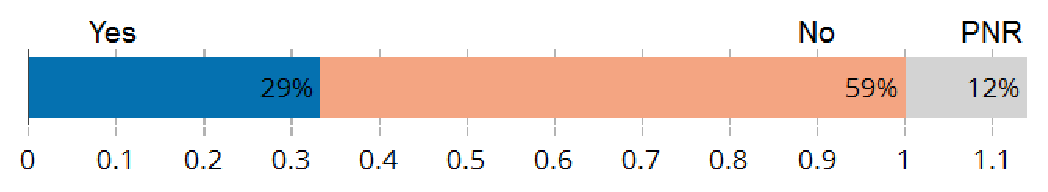
\includegraphics[width=0.9\columnwidth]{Images_EPS/diesel_catch_up_trim.eps}
\caption{Approval of a catching-up of the diesel tax.}
\label{fig:diesel}
\end{figure}

The strong opposition of the Yellow Vests against energy taxes did not only lead the government to reverse the planned carbon tax trajectory. The additional tax increases initially scheduled for diesel --- to catch-up with the currently higher rates imposed on gasoline despite diesel's high social cost from air pollution  --- have also been abandoned.\footnote{Three increases of +0.026\euro{}/L were initially scheduled for January 2019, 2020 and 2021.}  In our survey, we ask respondents whether they would therefore accept an increase in diesel tax to catch up with that of gasoline. As illustrated by Figure \ref{fig:diesel}, 59\% of respondents answer they would not, while 29\% say they would (12\% ``PNR''). Among the 57\% of households who own a diesel vehicle, the opposition augments to 80\%. The geographic difference is also striking as 73\% of rural households would be opposed, vs. only 40\% of those living in the Paris agglomeration. As shown in our online Appendix 3.1, these two determinants appear as the most important divides with respect to diesel taxation.
% DONE: "persist when controlling for many other criteria and clearly appear, along with political orientation," -> "appear" 

% The additional tax increases initially scheduled for diesel (+0.026\euro{}/L) have also been abandoned. Diesel price was indeed supposed to rise more rapidly, in order to progressively catch-up with the currently higher tax imposed on gasoline. This historical advantage was considered by the government as a bad signal given the social costs of diesel from air pollution.

% Done : partie "Shale gas exploitation" supprimée (ci dessous en commentaire).

%         \subsubsection{Shale gas exploitation}


% The energy transition implies a shift away from fossil fuels, but it is sometimes argued that, at least in the short run, a substitution from coal to shale gas would reduce emissions as the former pollutes less than the latter. As France holds among the largest reserves of shale gas in Europe, its exploitation could be exported and \textit{possibly} substitute for more carbon intensive fuels.\footnote{See \citet{eia_shale_2013} for an assessment of recoverable reserves, and \citet{saussey_2018} for a nuanced view on the prospects for such exploitation in France.} Before asking for approval of shale gas exploitation, we first provide respondents with trade-offs between the possible climate benefits relative to coal and the potential negative effects on water quality at the local level. Then, using respondents' zipcode, we inform them whether their district would possibly be concerned by shale gas exploitation.\footnote{Source: exploitation and exploration permits, and exploration permit applications in 2011, as reported by \href{http://www.lefigaro.fr/societes/2011/10/04/04015-20111004ARTFIG00465-gaz-de-schiste-total-veut-des-explications.php}{Le Figaro}. Original source is \href{http://www.minergies.fr/fr/cartographie}{Direction Générale de l'Énergie et du Climat}, but the archive is not accessible.} 59\% of respondents declare being opposed to exploitation, while 16\% are in favor. As shown in our online Appendix, acceptance (defined as approval or ``PNR'') appears lower by 5 p.p. \textit{ceteris paribus} when the district is concerned. When asked about the main benefit of shale gas exploitation, 26\% answer it would ``create jobs and boost employment in the districts concerned'', 18\% that it would limit climate change, and none of these reasons for the other 56\%. Finally, 25\% of respondents think it is valid to say that shale gas exploitation would limit climate change, as ``any decrease in emissions goes in the right direction'', while 43\% think it is not, as ``emissions should be stopped, not just slowed down''. % DONE higher ... not concerned -> lower ... concerned / dept -> district
% % Among those favorable to exploitation, 48\% invoke job creation, 48\% climate change and 4\% are favorable for other reasons. 

% % Source: exploitation and exploration permits, and exploration permit applications in 2011, as reported by \href{http://www.lefigaro.fr/societes/2011/10/04/04015-20111004ARTFIG00465-gaz-de-schiste-total-veut-des-explications.php}{Le Figaro}, as well as the associations \href{https://nonaugazdeschistelyon.files.wordpress.com/2011/03/france_tm_01_2012.pdf}{Non au gaz de schiste} and \href{https://stopgazdeschiste.org/cartes-de-demande-de-permis/}{Stop gaz de schiste}. Original source is \href{http://www.minergies.fr/fr/cartographie}{Direction Générale de l'Énergie et du Climat}, but the archive is not accessible.

% \begin{figure}[!htbp]
% \centering
% 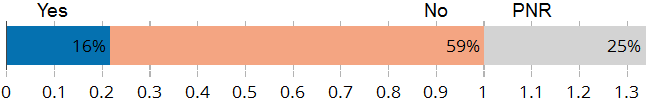
\includegraphics[width=0.9\columnwidth]{Images_EPS/shale_val_nolegend_trim.eps}
% \caption{Approval of shale gas extraction in France.}
% \label{fig:shale}
% \end{figure}


% Note: sondage BVA -> 77% des français pensent qu'une meilleure protection de l'nevironnement passe avant tout par Un changement profond des mentalités individuelles, 21% par des lois et des réglementations strictes contre les abus (1% NSP).

\section{Determinants of Attitudes\label{sec:determinants}}

To understand what factors foster environmentally-friendly attitudes, we explore the socio-demographic determinants of attitudes over CC, the correlations between knowledge and perception of CC, and how these attitudes over CC as well as socio-demographics shape preferences for policies. 

    \subsection{Attitudes over climate change}\label{sec:determinants_attitudes_CC}

% DONE: virer "These include causal knowledge (notably about the anthropogenic origin), basic knowledge (about climate science), effects knowledge (about the impacts) and action-related knowledge (about the factors of CC)."
Table \ref{tab:determinants_attitudes_CC} shows the main socio-demographic determinants of different attitudes towards CC: the knowledge that CC is anthropogenic (columns 1-3), an index of knowledge about CC (4) and the perception that CC is ``disastrous'' or ``cataclysmic'' (5-6). To build the index of knowledge, we aggregate different variables corresponding to the different kinds of knowledge about CC identified by \citet{kiel_einfuhrung_2002} \citep[see also][for a summary]{hoppe_what_2018}. 

We first compute a score for the question asking the emission target p.c. required to limit CC (see section \ref{subsec:knowledge}). Denoting $t$ as the respondent's answer (from 0 to 10 tCO$_2$/yr), we define the score as:

\begin{equation}
\textnormal{score emission target}=\begin{cases}
3 & \text{if }t\leq2\\
2 & \text{if }t\in\left[3;4\right]\\
1 & \text{if }t\in\left[5;6\right]\\
0 & \text{if }t\geq7
\end{cases}
\end{equation}

\noindent and we then aggregate this score with other answers:

\begin{align}
\textnormal{knowledge} = & \; 3\cdot \textnormal{CC anthropogenic}-2\cdot \textnormal{CC doesn't exist} \nonumber \\ & + \textnormal{ score factors}+\textnormal{score emission target} \label{eq:knowledge2}
\end{align}

where ``score factors'' is the sum of correct answers to factors of CC (see Figure \ref{fig:factors}), and the two first variables in the formula are dummies. The relative weights of the variables correspond to the loadings of a one-factor analysis, ensuring that our index captures the most determinant elements of knowledge.\footnote{See online Appendix 4 for more details.} The original index ranges from $-$2 (no respondent) to +13 (22 respondents), and has quartiles of 6, 8 and 9. In the regressions, we normalize this index by subtracting the mean (7.6) and dividing by the standard deviation (2.5). Finally, we run OLS regressions of the three attitudes over CC on various socio-demographics, household characteristics, and political orientation. We report only the most relevant variables, but describe the entire list of covariates in Appendix \ref{app:covariates}. We confirm that logistic regressions yield similar results (see online Appendix 5).


\begin{table*}[!htbp] \centering 
  \caption{Determinants of attitudes towards climate change (CC).} 
  \label{tab:determinants_attitudes_CC} 
\makebox[\textwidth][c]{ \begin{tabular}{@{\extracolsep{5pt}}lcccccc} 
\\[-1.8ex]\hline 
\hline \\[-1.8ex] 
\\[-1.8ex] & \multicolumn{3}{c}{CC is anthropogenic} & Knowledge about CC & \multicolumn{2}{c}{CC is disastrous} \\ 
\\[-1.8ex] & (1) & (2) & (3) & (4) & (5) & (6)\\ 
\hline \\[-1.8ex] 
 Interest in politics (0 to 2) & 0.032$^{**}$ &  &  & 0.137$^{***}$ & 0.051$^{***}$ &  \\ 
  & (0.013) &  &  & (0.028) & (0.014) &  \\ 
  Ecologist & 0.135$^{***}$ &  &  & 0.404$^{***}$ & 0.192$^{***}$ &  \\ 
  & (0.024) &  &  & (0.053) & (0.027) &  \\ 
  Yellow Vests: PNR & $-$0.098$^{***}$ &  &  & $-$0.142$^{**}$ & $-$0.093$^{***}$ &  \\ 
  & (0.033) &  &  & (0.071) & (0.036) &  \\ 
  Yellow Vests: understands & $-$0.038$^{*}$ &  &  & $-$0.100$^{**}$ & $-$0.051$^{**}$ &  \\ 
  & (0.022) &  &  & (0.048) & (0.024) &  \\ 
  Yellow Vests: supports & $-$0.098$^{***}$ &  &  & $-$0.223$^{***}$ & $-$0.061$^{**}$ &  \\ 
  & (0.024) &  &  & (0.051) & (0.026) &  \\ 
  Yellow Vests: is part & $-$0.207$^{***}$ &  &  & $-$0.498$^{***}$ & $-$0.105$^{**}$ &  \\ 
  & (0.043) &  &  & (0.093) & (0.047) &  \\ 
  Left-right: Extreme-left & 0.111$^{**}$ &  & 0.109 & 0.295$^{**}$ & 0.075 & 0.005 \\ 
  & (0.056) &  & (0.077) & (0.122) & (0.062) & (0.084) \\ 
  Left-right: Left & 0.074$^{***}$ &  & 0.070 & 0.137$^{**}$ & 0.099$^{***}$ & $-$0.025 \\ 
  & (0.027) &  & (0.046) & (0.059) & (0.030) & (0.051) \\ 
  Left-right: Center & 0.013 &  & 0.039 & 0.093 & 0.021 & $-$0.089$^{*}$ \\ 
  & (0.030) &  & (0.044) & (0.065) & (0.033) & (0.048) \\ 
  Left-right: Right & $-$0.029 &  & $-$0.017 & $-$0.039 & $-$0.023 & $-$0.143$^{***}$ \\ 
  & (0.029) &  & (0.045) & (0.062) & (0.032) & (0.049) \\ 
  Left-right: Extreme-right & $-$0.014 &  & $-$0.019 & $-$0.117 & 0.025 & $-$0.086 \\ 
  & (0.034) &  & (0.055) & (0.074) & (0.037) & (0.060) \\ 
  Diploma: \textit{CAP} or \textit{BEP} & 0.040$^{*}$ &  & 0.033 & $-$0.004 & $-$0.014 & $-$0.010 \\ 
  & (0.022) &  & (0.023) & (0.049) & (0.025) & (0.025) \\ 
  Diploma: \textit{Baccalauréat} & 0.065$^{**}$ &  & 0.115$^{***}$ & 0.145$^{**}$ & 0.030 & 0.133$^{***}$ \\ 
  & (0.027) &  & (0.028) & (0.058) & (0.029) & (0.031) \\ 
  Diploma: Higher & 0.086$^{***}$ &  & 0.159$^{***}$ & 0.266$^{***}$ & 0.096$^{***}$ & 0.240$^{***}$ \\ 
  & (0.027) &  & (0.027) & (0.059) & (0.030) & (0.030) \\ 
  Diploma $\times$ Left-right &  &  & $-$0.005 &  &  & $-$0.005 \\ 
  &  &  & (0.008) &  &  & (0.009) \\ 
  Diploma $\times$ Left-right: Indeterminate &  &  & 0.013 &  &  & $-$0.027$^{*}$ \\ 
  &  &  & (0.014) &  &  & (0.015) \\ 
  Age: 25 -- 34 & 0.050 & $-$0.030 &  & 0.128 & 0.021 &  \\ 
  & (0.041) & (0.032) &  & (0.089) & (0.045) &  \\ 
  Age: 35 -- 49 & 0.002 & $-$0.088$^{***}$ &  & 0.092 & 0.032 &  \\ 
  & (0.041) & (0.029) &  & (0.089) & (0.045) &  \\ 
  Age: 50 -- 64 & 0.009 & $-$0.092$^{***}$ &  & 0.069 & $-$0.032 &  \\ 
  & (0.044) & (0.029) &  & (0.096) & (0.049) &  \\ 
  Age: $\geq$ 65 & $-$0.106$^{**}$ & $-$0.197$^{***}$ &  & $-$0.052 & $-$0.092 &  \\ 
  & (0.053) & (0.029) &  & (0.114) & (0.058) &  \\ 
  Income (k\euro{}/month) & $-$0.008 &  &  & $-$0.018 & $-$0.012 &  \\ 
  & (0.008) &  &  & (0.017) & (0.009) &  \\ 
  Sex: Male & $-$0.023 &  &  & 0.156$^{***}$ & $-$0.004 &  \\ 
  & (0.018) &  &  & (0.039) & (0.020) &  \\ 
  Size of town (1 to 5) & 0.004 &  &  & $-$0.003 & 0.006 &  \\ 
  & (0.008) &  &  & (0.017) & (0.009) &  \\ 
  Frequency of public transit & 0.016$^{**}$ &  &  & 0.045$^{***}$ & 0.007 &  \\ 
  & (0.007) &  &  & (0.016) & (0.008) &  \\ 
 \hline \\[-1.8ex] 
Additional covariates & \checkmark &  &  & \checkmark & \checkmark &  \\  &  &  &  &  &  &  \\ 
Observations & 3,002 & 3,002 & 3,002 & 3,002 & 3,002 & 3,002 \\ 
R$^{2}$ & 0.104 & 0.021 & 0.037 & 0.156 & 0.118 & 0.048 \\ 
\hline 
\hline \\[-1.8ex] 
\textit{Note:}  & \multicolumn{6}{r}{$^{*}$p$<$0.1; $^{**}$p$<$0.05; $^{***}$p$<$0.01} \\ 
\end{tabular} 
}{\\ $\quad$ \\                \footnotesize \textsc{Note:} Standard errors are reported in parentheses. Interaction term is computed using numeric variables. Omitted modalities are: \textit{Yellow Vests: opposes}, \textit{Left-right: Indeterminate}, \textit{Diploma: Brevet or no diploma}, \textit{Age: 18 -- 24}. Additional covariates are defined in \ref{app:covariates}. }                \end{table*}  

% concerned attitudes -> concern DONE
%plays a ``pro-climate'' role, though a less important one
% DONE: orientation shapes different attitudes in a consistent manner => "Political orientation shapes attitudes" instead of "Political orientation shapes different attitudes"? pck sinon ça peut se comprendre différemment: l'orientation politique façonne des attitudes de façon différente d'une manière cohérente (ce qui ne veut rien dire, je te l'accorde)
The best predictors of attitudes over CC corresponds to political orientation, and in particular identifying as an ecologist, one's positioning towards the Yellow Vests, and left-right leaning. Political orientation shapes attitudes in a consistent manner: being ecologist, more left-wing or less supportive of the Yellow Vests is always associated with higher ``concern over CC'', i.e. better knowledge and higher pessimism. Interest into politics (measured on a scale ``almost not''/``a little''/``a lot'') also leads to higher concern, but to a lesser extent. Two observations on the left-right leaning deserve comment. First, the 40\% of people indeterminate relative to this spectrum (see Appendix \ref{app:stats_des} for the descriptive statistics) have attitudes close to the center-right. Second, the variations predicted in the dependent variables are as high across the Yellow Vests positionings as across the traditional left-right spectrum. For instance, knowledge about CC is \textit{ceteris paribus} lower by 0.50 standard deviation (s.d.) for people part of the movement than for those who oppose it, which is comparable to the spread of 0.41 s.d. between extreme-right and extreme-left people (4). 

% DONE: In general -> On average
Two socio-demographics are also consistently related to attitudes over CC: age and level of education. On average, the younger and the more educated one is, the more one is concerned by CC. People aged 18-24 may appear to have slightly lower knowledge and lower pessimism than people of prime age \textit{ceteris paribus}, in columns (1,4,5); but this is because their concern is mostly captured by the employment status modality ``student'', not shown in the table. Overall, the generation with the least concern is undeniably those aged over 65. For instance, without any control, they are 20 percentage points (p.p.) less likely to believe that CC is anthropogenic than young adults (2) --- though most of this effect is explained by a lower level of education (1). Another finding is that men have a higher knowledge than women by 0.16 s.d. \textit{ceteris paribus} (4), but their perception of the severity of CC is virtually the same (5). Finally, other characteristics have smaller or even insignificant effects. 

Although the determinants we find are broadly consistent with those elicited in the literature \citep{upham_public_2009,whitmarsh_scepticism_2011, ademe_representations_2018},\footnote{See also \citet{capstick_international_2015} for trends in attitudes.} we do not encounter the political polarity which characterizes the United States. Indeed, \citet{kahan_polarizing_2012} argue that American people ``tend to form perceptions of societal risks that cohere with values characteristic of groups with which they identify'' (this is the cultural cognition thesis), rather than through an assessment of the scientific evidence they encounter (the science comprehension thesis). It is crucial to know whether people neglect climate science in such a way, as this would mean that a media campaign would have little effect on people's assimilation of climate science. \citet{kahan_polarizing_2012} and \citet{mccright_politicization_2011} provide evidence for cultural cognition by showing that education has little effect on perceived risk or knowledge about CC, while the interaction between education and political orientation has a significant effect.\footnote{\citet{funk_politics_2016} also report that Republicans are equally distrustful of climate scientists' integrity whatever their level of education, while the distrust vanishes for Democrats with higher degrees. The mechanism of the interaction is documented by \citet{ehret_partisan_2018} and \citet{van_boven_psychological_2018}: people form beliefs through partisan cues, by adopting views expressed by political figures of the party they identify and rejecting positions from the other party.} We assess whether such interaction appears in the French context, by studying the interaction between the higher degree obtained and the left-right political leaning (columns 4, 6). We find no significant interaction, and obtain the same nil result when replacing the traditional left-right scale by the Yellow Vests positioning, and/or the higher degree by knowledge about CC (see online Appendix 6). This lack of evidence suggests that the public debate over CC is less polarized in France than in the US,\footnote{A finding reminiscent of \citet{ziegler_political_2017}, who studies Germany.} and that the knowledge and perception of many French people could change with better access to information over CC. % DONE: référence to Ziegler added

% La phrase "It is crucial..." pourrait être supprimée et remplacée par une phrase plus courte à la fin de ce paragraphe.


%Although the determinants we find are broadly consistent with those elicited in the literature \citep{whitmarsh_scepticism_2011, ademe_representations_2018}, we do not retrieve the political polarity which characterizes the United States. Indeed, a series of paper have shown that not only do the American political cleavage translate into sharp contrasts in attitudes over CC, but that the cleavage also determines how other factors shape these attitudes. \citet{kahan_polarizing_2012} argue that American people ``tend to form perceptions of societal risks that cohere with values characteristic of groups with which they identify'' (this is the cultural cognition thesis), rather than through an assessment of the scientific evidence they encounter (the science comprehension thesis). It is crucial to know whether people neglect climate science in such a way, as this would mean that media campaign would have little effects on people's assimilation of climate science. \citet{kahan_polarizing_2012} and \citet{mccright_politicization_2011} provide evidence for the cultural cognition thesis using similar methods: they show that education has little effect on perceived risk or on knowledge of CC, while the interaction between education and political orientation has. \citet{funk_politics_2016} also report that Republicans are equally distrustful of climate scientists' integrity whatever their level of education, while the distrust vanishes for Democrats with higher degrees. The mechanism of the interaction is documented by \citet{ehret_partisan_2018} and \citet{van_boven_psychological_2018}: people form beliefs through partisan cues, by adopting views expressed by political figures of the party they identify and rejecting positions from the other party. We assess whether such interaction appears in the French context, by studying the interaction between the higher degree obtained and the left-right political leaning (columns 4, 6). We find no significant interaction, and obtain the same nil result when replacing the traditional left-right scale by the Yellow Vests positioning, and/or (in 6) the higher degree by knowledge on CC. This lack of evidence suggests that the public debate over CC is less polarized in France than in the US, and that the knowledge and perception of many French people could change, had they access to better information over CC. 
% Although people of both parties may have comparable underlying beliefs on what the scientific consensus affirms, whose correctness increase with their education \citep{kahan_climate-science_2015}, the position they defend socially is in fact determined by the polarity between the left and the right over climate issues, and they adopt the scientific consensus only when it coheres with their partisan identity. 

% cite Capstick et al. 2015 on polarization and Brulle et al 2012 on factors of concern in CC: economic factors and elite cues there has been growing political polarization in the United States, with right‐of‐center voters growing increasingly skeptical, compared to left‐of‐center voters. This is consistent with pervasive ‘confirmation bias’ (the propensity to seek out and believe information that confirms existing views140) and interest‐based efforts to shape public opinion. Capstick et al. 2015

Figure \ref{fig:correlations} gives a sense of the shift in the perception and support for climate policies that could follow an information campaign, as it shows the correlations between attitudes over CC, climate policies, and socio-demographics. Knowledge is highly correlated with the perceived gravity of CC (correlation of 0.43), and both of these variables are in turn well correlated with the readiness to adopt an ecological lifestyle and to the number of climate policies (of Figure \ref{fig:policies}) supported (correlations around 0.3). The acceptance of our Tax \& Dividend is less correlated with attitudes (at 0.1-0.2), as the support for this policy is already low. Still, the positive correlation between knowledge and support for other climate policies is an encouraging prospect for an information campaign about CC and even more so since we did not find evidence that partisanship would lead to the dismissal of scientific discourse. Finally, as previously seen, diploma and age are quite correlated with attitudes, though these correlations are below those between attitudes over CC and over policies, at 0 to 0.2. 
% Utiliser MNL pour traiter PNR de manière distincte (sur le choix MNP/MNL, cf. \citet{dow_endersby_2004}).

\begin{figure}[!htbp]
\centering
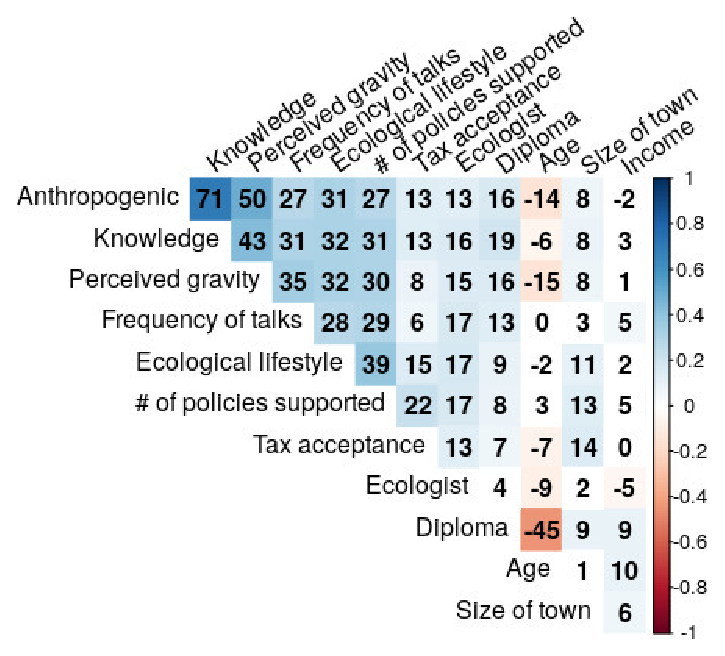
\includegraphics[width=0.95\columnwidth]{Images_EPS/correlation_matrix2.eps}
\caption{Correlations between attitudes over climate change, climate policies and socio-demographics (in \%).}
\label{fig:correlations}
\end{figure}

    \subsection{Attitudes over policies}\label{sec:determinants_attitudes_policies}

%In section \ref{sec:attitudes_carbon_tax} and \ref{sec:attitudes_other_policies} we have described how people respond on average to various environmental policies.
To better understand the heterogeneity in people's support, we regress several indicators of attitudes towards climate policies on respondents' characteristics. Table \ref{tab:politiques_env} reports the results for the acceptance of our Tax \& Dividend (columns 1-2) and the readiness to adopt an ecological lifestyle (6) in the case that the richest were contributing, efforts were shared globally, and alternatives were developed. We also use the eight policies proposed in Figure \ref{fig:policies} in our dependent variables: column 3 studies the share of policies approved while column 4 features the preference for norms vs. taxes within the policies. Similarly, column 5 uses six measures of Figure \ref{fig:recycling} to define an index of preference for earmarking vs. transfers. Indexes for these preferences are constructed as follows:

\begin{align}
\textnormal{Norms vs. taxes} = \sum_{p \in \textnormal{norms}} \textnormal{score}_{p} - \sum_{p \in \textnormal{taxes}}  \textnormal{score}_{p}
\label{eq:norms_vs_taxes}
\end{align}

\noindent
where the score of each measure corresponds to a grade between $-$2 (for a ``Not at all'' answer) and 2 (for ``Yes, completely''). We proceed similarly for earmarking vs. transfers, and describe the categorization of measures in Appendix \ref{app:measures}. Again, we normalize these two indexes by subtracting the mean (2.8 for norms vs. taxes, 1.4 for earmarking vs. transfers) and dividing by the standard deviation (3.3 and 3.1 respectively). Tables 3.2 and 3.3 in online Appendix provide the analysis of the determinants of acceptance for each of the eight policies and nine revenue recycling. The results are overall very similar to those provided by the more synthetic indicators presented here.

% Done : ajout des deux dernières phrases pour renvoyer vers les tables 4.3 et 4.4


\begin{table*}[!htbp] \centering 
  \caption{Determinants of attitudes towards climate policies} 
  \label{tab:politiques_env} 
\makebox[\textwidth][c]{ \begin{tabular}{@{\extracolsep{5pt}}lcccccc} 
\\[-1.8ex]\hline 
\hline \\[-1.8ex] 
\\[-1.8ex] & \multicolumn{2}{c}{Acceptance of} & Share of policies & Norms & Earmarking & Ecological \\ \\[-1.8ex] & \multicolumn{2}{c}{Tax \& dividend} & approved & vs. taxes & vs. transfers & lifestyle \\ 
\\[-1.8ex] & (1) & (2) & (3) & (4) & (5) & (6)\\ 
\hline \\[-1.8ex] 
 Knowledge about CC & 0.029$^{***}$ & 0.048$^{***}$ & 0.044$^{***}$ & 0.024 & 0.131$^{***}$ & 0.103$^{***}$ \\ 
  & (0.009) & (0.009) & (0.005) & (0.020) & (0.020) & (0.009) \\ 
  CC is disastrous & 0.022 & 0.037$^{**}$ & 0.081$^{***}$ & 0.125$^{***}$ & 0.156$^{***}$ & 0.142$^{***}$ \\ 
  & (0.018) & (0.018) & (0.010) & (0.040) & (0.039) & (0.018) \\ 
  Interest in politics (0 to 2) & $-$0.019 &  & 0.034$^{***}$ & $-$0.010 & 0.053$^{*}$ & 0.026$^{**}$ \\ 
  & (0.013) &  & (0.007) & (0.029) & (0.028) & (0.013) \\ 
  Ecologist & 0.126$^{***}$ &  & 0.082$^{***}$ & $-$0.134$^{**}$ & 0.249$^{***}$ & 0.149$^{***}$ \\ 
  & (0.024) &  & (0.013) & (0.056) & (0.054) & (0.025) \\ 
  Yellow Vests: PNR & $-$0.021 &  & $-$0.052$^{***}$ & 0.007 & $-$0.110 & $-$0.079$^{**}$ \\ 
  & (0.032) &  & (0.018) & (0.073) & (0.071) & (0.033) \\ 
  Yellow Vests: understands & $-$0.144$^{***}$ &  & $-$0.029$^{**}$ & $-$0.056 & $-$0.091$^{*}$ & $-$0.013 \\ 
  & (0.022) &  & (0.012) & (0.050) & (0.049) & (0.022) \\ 
  Yellow Vests: supports & $-$0.222$^{***}$ &  & $-$0.048$^{***}$ & $-$0.131$^{**}$ & $-$0.142$^{***}$ & $-$0.023 \\ 
  & (0.023) &  & (0.013) & (0.053) & (0.052) & (0.024) \\ 
  Yellow Vests: is part & $-$0.214$^{***}$ &  & $-$0.084$^{***}$ & $-$0.252$^{***}$ & $-$0.175$^{*}$ & $-$0.037 \\ 
  & (0.043) &  & (0.023) & (0.097) & (0.095) & (0.043) \\ 
  Left-right: Extreme-left & $-$0.040 &  & 0.025 & $-$0.285$^{**}$ & 0.167 & 0.047 \\ 
  & (0.056) &  & (0.031) & (0.127) & (0.124) & (0.056) \\ 
  Left-right: Left & 0.072$^{***}$ &  & $-$0.005 & $-$0.137$^{**}$ & 0.002 & 0.028 \\ 
  & (0.027) &  & (0.015) & (0.061) & (0.060) & (0.027) \\ 
  Left-right: Center & 0.051$^{*}$ &  & 0.011 & $-$0.051 & 0.051 & 0.095$^{***}$ \\ 
  & (0.030) &  & (0.016) & (0.068) & (0.066) & (0.030) \\ 
  Left-right: Right & $-$0.022 &  & 0.008 & 0.030 & 0.064 & 0.005 \\ 
  & (0.028) &  & (0.016) & (0.065) & (0.063) & (0.029) \\ 
  Left-right: Extreme-right & $-$0.041 &  & $-$0.028 & 0.055 & 0.009 & 0.014 \\ 
  & (0.034) &  & (0.018) & (0.077) & (0.075) & (0.034) \\ 
  Diploma (1 to 4) & $-$0.006 & $-$0.001 & 0.005 & 0.006 & 0.017 & $-$0.008 \\ 
  & (0.009) & (0.008) & (0.005) & (0.020) & (0.020) & (0.009) \\ 
  Age: 25 -- 34 & $-$0.047 & $-$0.099$^{***}$ & $-$0.023 & 0.038 & $-$0.159$^{*}$ & 0.032 \\ 
  & (0.041) & (0.032) & (0.022) & (0.093) & (0.090) & (0.041) \\ 
  Age: 35 -- 49 & $-$0.047 & $-$0.089$^{***}$ & $-$0.017 & 0.189$^{**}$ & $-$0.002 & 0.039 \\ 
  & (0.040) & (0.030) & (0.022) & (0.092) & (0.089) & (0.041) \\ 
  Age: 50 -- 64 & $-$0.054 & $-$0.114$^{***}$ & $-$0.010 & 0.322$^{***}$ & $-$0.058 & 0.049 \\ 
  & (0.044) & (0.031) & (0.024) & (0.100) & (0.097) & (0.044) \\ 
  Age: $\geq$ 65 & $-$0.066 & $-$0.100$^{***}$ & $-$0.009 & 0.370$^{***}$ & $-$0.056 & 0.008 \\ 
  & (0.052) & (0.032) & (0.028) & (0.118) & (0.115) & (0.052) \\ 
  Income (k\euro{}/month) & 0.006 & 0.001 & 0.009$^{**}$ & 0.014 & 0.031$^{*}$ & $-$0.004 \\ 
  & (0.008) & (0.005) & (0.004) & (0.018) & (0.017) & (0.008) \\ 
  Sex: Male & $-$0.053$^{***}$ & $-$0.074$^{***}$ & $-$0.017$^{*}$ & $-$0.028 & $-$0.004 & $-$0.063$^{***}$ \\ 
  & (0.018) & (0.017) & (0.010) & (0.040) & (0.039) & (0.018) \\ 
  Size of town (1 to 5) & 0.019$^{**}$ & 0.033$^{***}$ & 0.0002 & 0.009 & $-$0.003 & $-$0.003 \\ 
  & (0.008) & (0.007) & (0.004) & (0.018) & (0.017) & (0.008) \\ 
  Frequency of public transit & $-$0.003 & 0.014$^{**}$ & $-$0.003 & 0.046$^{***}$ & 0.021 & 0.024$^{***}$ \\ 
  & (0.007) & (0.006) & (0.004) & (0.017) & (0.016) & (0.007) \\ 
 \hline \\[-1.8ex] 
Additional covariates & \checkmark & & \checkmark  & \checkmark & \checkmark & \checkmark  \\  &  &  &  &  &  &  \\ 
Observations & 3,002 & 3,002 & 3,002 & 3,002 & 3,002 & 3,002 \\ 
R$^{2}$ & 0.150 & 0.051 & 0.226 & 0.081 & 0.121 & 0.202 \\ 
\hline 
\hline \\[-1.8ex] 
\textit{Note:}  & \multicolumn{6}{r}{$^{*}$p$<$0.1; $^{**}$p$<$0.05; $^{***}$p$<$0.01} \\ 
\end{tabular} 
} \\ \quad \\ {\footnotesize \textsc{Note:} Standard errors are reported in parentheses. Omitted variables are \textit{Yellow Vests: opposes}, \textit{Age : 18 -- 24} and \textit{Left-right: Indeterminate}. Additional covariates are defined in \ref{app:covariates}.} \end{table*} 

As suggested by the correlation matrix of section \ref{sec:determinants_attitudes_CC}, knowledge about CC and the conviction that it would be disastrous positively affect the approval of climate policies, \textit{ceteris paribus}. Excluding the (endogenous) variables describing political orientation, an increase in knowledge by 1 s.d. would induce a lower likelihood to reject Tax \& Dividend by 5 p.p. (column 2). The effect of these variables is even stronger when considering the share of policies approved: controlling for socio-demographics, an increase in knowledge by 1 s.d. is associated with an additional approval of 6 p.p. while the conviction that CC is disastrous increases it by 9 p.p. (see online Appendix 3.4). Beyond the strong correlation we previously found, these results confirm that increasing climate awareness could significantly increase the support for climate policies. % DONE: clearly show ... would -> confirm ... could (c'est pas causal)

%  This result confirms previous evidence from other countries, such as \citet{thalmann_public_2004} and \citet{bornstein_lanz_2008} in Switzerland.
% positioning towards ecologists -> affiliation as an ecologist
% DONE: "Ecologists also display a higher relative preference for earmarking, consistent with a willingness to increase environmental spending in general. Conversely, since Yellow Vests supporters are overall less likely to accept environmental policies including norms, their relative preference for norms against taxes is lower than average. They also have a higher relative preference for transfers vs. earmarking compared to other households, consistent with a lower willingness to pay to protect the environment and/or greater concerns regarding purchasing power."  -> "Ecologists (resp. the Yellow Vests supporters) being more (resp. less) favorable to environmental policies and spending, their relative preference for earmarking vs. transfers is higher (resp. lower) than average, while for both groups the relative preference for norms vs. taxes is lower than average."
% DONE: removed "who are not significantly less ready to adopt an ecological lifestyle"
Besides attitudes over CC, the two most critical determinants appear to be one's affiliation as an ecologist and one's position towards the Yellow Vests. All else equal, ecologists are more likely to accept Tax \& Dividend by 13 p.p., and more willing to approve other environmental policies by about 8 p.p. Conversely, holding other variables constant, people supporting the Yellow Vests are 22 p.p. more likely to reject Tax \& Dividend relative to those opposed to the movement. As shown in column 3, higher affinity with the Yellow Vests is also associated with less support for other climate policies. Ecologists (resp. the Yellow Vests supporters) being more (resp. less) favorable to environmental policies and spending, their relative preference for earmarking vs. transfers is higher (resp. lower) than average, while for both groups the relative preference for norms vs. taxes is lower than average. Also, ecologists' attitudes towards environmental policies translate into a higher willingness to adopt an ecological lifestyle (by 15 p.p.), but the opposite does not hold true for the Yellow Vests. Although this could signal some warm glow,\footnote{Here, ``warm glow'' refers to one's unintentional strategy to overestimate their virtue in order to derive satisfaction.} it also suggests that their strong rejection of environmental policies does not simply reflect lower concerns about the environment. Rather, the conditions of fairness embedded in our question could be critical for Yellow Vests to accept sacrifices. Their rejection could also reflect a deeper rejection of policies in general, due to a high distrust in the government --- documented in \citet{algan_et_al_19}. This interpretation echoes the recent findings of \citet{rafaty_perceptions_2018}, who shows that perceptions of corruption and political distrust negatively affect the stringency of climate policies. Finally, although the heterogeneity in responses is significant between these two groups, the ranking of the preferred option remains consistent: on average, both ecologists and supporters of the Yellow Vests favor norms over taxes and earmarking over transfers. 
% DONE: The conditions of fairness embedded in our question could be critical if Yellow Vests are to accept sacrifices. -> Rather, the conditions of fairness embedded in our question could be critical for Yellow Vests to accept sacrifices.

% Done ("consistently with a lower" -> "consistent with a lower")
% Done ("does not simply reflects from lower concerns" -> "does not simply reflect lower concerns")

% citer Rafaty et al (2018) ? On peut l'ajouter à la ref à Drews and van der Bergh, ou simplement substituer puisqu'on cite déjà ces auteurs à plusieurs reprises. La référence à Rafaty devrait suffire puisque c'est l'article le plus récent qui traite précisémment de ce sujet. On pourrait remplacer la dernière phrase par : "This interpretation echoes the recent findings of Rafaty (2018), who shows that perceptions of corruption and political distrust negatively affect the stringency of climate policies." => oui très bien

%Although this could to some extent reflect warm glow, it also suggests that their strong rejection of environmental policies does not simply follows from lower concerns about the environment: it could also translate a deeper rejection of policies in general, due to a high distrust in governments --- documented for instance in \citet{algan_et_al_19} --- as well as the necessity to meet the conditions mentioned in this question, in particular the sharing of efforts, the contribution of the richest and the development of alternatives.

% With respect to the Tax \& Dividend, the only significant effect is for the extreme-left, with a positive coefficient of 0.11 which partly compensates for the higher share of people supporting the Yellow Vests in this category (63\% support or are part), and whose attitude towards the environment might differ from other supporters of the movement. This result somewhat contrasts with literature that has shown evidence of greater support for climate policies from people on the left of the political spectrum \citep[see][for a review]{drews_van_der_bergh_2016}.
% DONE clear -> parallel / hardly -> not the most / puis plein d'autres changements
A parallel message from Table \ref{tab:politiques_env} is that the standard left-right spectrum is not the most relevant to understand attitudes towards environmental policies. None of our five left-right dummy variables are significantly correlated with the share of policies approved, and overall, attitudes vary much less along the left-right spectrum than along the Yellow Vests cleavage. That being said, Tax \& Dividend is still significantly more supported by people from the left (+7 p.p.) and the center (+5 p.p.) than by those indeterminate. This is in line with the literature (see e.g. \citealt{bornstein_lanz_2008,mccright_increasing_2013} or \citealt{drews_van_der_bergh_2016} for a review). Without controlling for other variables, we find that people that are most likely to accept the Tax \& Dividend in France are the ones affiliated with the center (+9 p.p. relative to ``Indeterminate''), and the least likely are those on the extreme-right (-15 p.p., see online Appendix 3.4), which may be driven by their respective support or rejection of the current government who tried to increase the carbon tax. Our results also show that people from the extreme-left and the center are the most likely to approve other environmental policies (+7 p.p.), while the least likely are those on the extreme-right ($-$6 p.p.). Still, these differences become small and not statistically significant when covariates are included. %Thus, consistent with \citet{ziegler_political_2017}, our results indicate that the correlation between political leaning and attitudes towards climate change exists but is to a large extent explained by other components of worldviews, such as environmental concerns.
% DONE À la relecture je comprends pas bien la phrase "Thus, consistent with Ziegler (2017), our results indicate that the correlation between political leaning and attitudes towards climate change exists but is to a large extent explained by other components of worldviews, such as environmental concerns." : c'est un peu évident que les attitudes climatiques sont mieux expliquées par les préoccupations environnementales que par l'orientation politique, non ? Aussi, on voit pas trop en quoi c'est "other" worldviews les préoccupations env par rapport aux attitudes climatiques (à moins que les worldviews soient l'orientation pol, mais alors préoccupation env c'est pas une "autre" worldview, c'est une "partie" de la worldview). Bref, je suis d'avis de reformuler. Peut-être simplement en : "Thus, consistent with Ziegler (2017), our results indicate that the correlation between political leaning and attitudes towards climate policies exists but is to a large extent explained by other components of worldviews, such as perceptions of CC." Une autre possibilité est de citer Ziegler ailleurs ou bien différemment : pour dire que Ziegler aussi trouve que le clivage gauche-droite est moins pregnant en Europe (Allemagne) qu'aux US concernant les attitudes sur le CC. -> Je viens de voir qu'il y a une "erreur" ici puisque Ziegler parle des attitudes vis à vis du CC et non des CP. Il faut donc formuler autrement ou le mettre ailleurs (même si le relecteur nous avait demandé de le mettre là, on peut lui expliquer que ça ne correspond pas tout à fait). Une manière de le reformuler serait : "Thus, while Ziegler shows that the correlation between political leaning and attitudes towards climate change is to a large extent explained by other components of worldviews, our findings extend this result to attitudes towards climate policies" mais en mieux dit. => pour moi ta nouvelle proposition le même problème que la précédente. Mais c'est vrai que la mienne ne convient pas non plus. Je propose de citer Ziegler ailleurs (cf. ci-dessus), d'expliquer au relecteur que Ziegler et Cherry ne sont pas pertinents, et de citer deux autres papiers: Bornstein & Lanz (08) et McCright et al. (13) dont un est dans Ecol Eco. En effet, le relecteur ne nous demande pas de rajouter des références ici, mais un peu plus haut dans le paragraphe, quand on dit que la gauche est plus pro pol climatiques. -> Ok très bien

% Done : ("people most likely" -> "people who are most likely")
% Done : ("(-15 p.p.)" -> "(-15 p.p., see online appendix, Table 2.3)") 

Besides political attitudes, we also observe heterogeneity in people's responses along socio-demographic lines. As in attitudes over CC, age plays a role, as 18-24 are about 10 p.p. more likely to accept the Tax \& Dividend (column 2). Still, controlling for knowledge, political attitudes and other variables, this effect is reduced by half. Similarly, more educated people tend to be more open to environmental policies \citep[as previously found by][]{thalmann_public_2004}, but this effect becomes insignificant once age dummies are included as covariates. Furthermore, we find little effect of income on attitudes towards climate policies, a result that confirms that of \citet{thalmann_public_2004} in Switzerland. Using our full set of controls, the most significant variables differ from the main factors of attitudes over CC: these significant variables are size of town \citep[city dwellers being more favorable to environmental policies, as in][]{thalmann_public_2004}, and sex (males being less favorable). Although men have a higher knowledge about CC than women on average, this does not translate into higher pessimism (see section \ref{sec:determinants_attitudes_CC}), and it even coincides with lower support for climate policies. This phenomenon is consistent with the findings of \citet{stern_value_1993} and \citet{hampel_gender_1996} that women are more attentive to links between the environment and things they value, even if they share the same values and beliefs as men. Difference in perception of CC's impact on oneself could explain women's higher support for climate policies, even given a lower factual knowledge. % DONE: could thus explain -> could explain

% This shows that, despite the positive correlation between knowledge and support for policies, the latter has its own determinants, which may act on the opposite direction than with the former. The most compelling case is that of sex: although men have on average a higher knowledge over CC than women, this does not translate into higher pessimism

%Previous studies have examined the factors explaining differences in attitudes towards environmental policies. \citet{stern_value_1993} find that women --- from a sample of college students --- are more likely to believe they can be harmed by environmental problems, but the value they assign to these beliefs does not significantly differ from men. Difference in beliefs with respect to the impact on oneself could thus explain the higher willingness of women to accept environmental policies. \citet{thalmann_public_2004} shows that people living in larger municipalities and with higher education are more favorable to carbon taxation in Switzerland, but he finds no significant relation with income. Our results confirm his findings on the income and geographical dimensions for France. Once controlled for age, we find however no evidence of a positive effect of diploma, although knowledge about CC significantly increases the chances to accept Tax \& Dividend and other environmental policies.

% Drews and van der Bergh: références supplémentaires sur les effets redistributifs et leur importance pour l'acceptation

% Lam (2014) cité par Drews and van der Bergh semble montrer que les enquêtes rendant les coûts des politiques saillant reçoivent moins de support.

% Jagers et Hammar (2009) cité par Drews and van der Bergh semblent montrer que les gens sous-estiment les coûts cachés des subventions et sur-estiment les coûts des taxes.

% Shwom et al (2010) cité par Drews and van der Bergh semblent montrer qu'aux Etats-Unis les gens utilisent l'impact sur l'économie et l'emploi comme argument contre les politiques environnementales. L'existence de gagnants et perdant apparaît aussi comme un élément essentiel de leur acceptation/rejet. -> petit sample et pas représentatif 2 états américains (Michigan et Virginie).

% Corrélation entre positionnement vis-à-vis de la taxe carbone et variables socio-démographiques : d’après Kallbekken & Aasen 2010 les papiers suivant traitent de la question : Eriksson et al. (2006), Fujii et al. (2004), Jakobsson et al. (2000), Loukopoulos et al. (2005) -> tout ça traite des péages urbains

\section{Conclusion}\label{sec:conclusion}

%Despite a social movement against the carbon tax, French people appear mostly aware and concerned about climate change. Their rejection should therefore not be taken as a low willingness to act for the environment, but rather as a perceived inadequacy between current carbon taxation and the fight for the climate. As shown in our companion paper \citet{douenne_can_2019}, people's beliefs about carbon taxation are largely biased, and these biases are well anchored, making it unlikely that carbon taxation be peacefully reintroduced in the short-run.

%The large opposition towards the French carbon tax is not necessarily incompatible with the call for more efforts to tackle climate change. Our results indicate that the low support encountered by carbon taxation is due to several barriers --- such as distributive concerns, inefficacy and lack of alternatives --- that could be partly alleviated with specific revenue uses.
% non-market climate policies,
Despite a social movement against the carbon tax, French people appear mostly aware and concerned about climate change. Their rejection should therefore not be taken as a low willingness to act for the environment, but rather as a perceived inadequacy between current carbon taxation and the fight for the climate. Our results identify several barriers --- distributive concerns, inefficacy and lack of alternatives --- that could be partly alleviated with specific complementary policies. In particular, French people favor investments in green infrastructures that provide them with alternatives and foster the energy transition. They also appear willing to accept certain norms as well as Pigouvian taxes if these target specific behaviors (or populations) such as air travel. The heterogeneity in people's attitudes is significant, but the relative ranking of the different policy options are in general consistent across groups of population, suggesting the following paths towards a successful ecological transition.
% appears important -> is significant
%possible avenues for a democratic energetic and ecological transition.


%Thus, our survey suggests the following paths forward for successful reforms. 
First and foremost, a massive and long-lasting information campaign could be launched to improve knowledge about climate change and climate policies. Indeed, higher knowledge is clearly associated with higher concern for CC and higher support for climate policies. Second, as people mostly favor policies that provide alternatives to fossil fuels, the government could develop such policies as a substitute to a carbon tax: investments, subsidies, and regulations in favor of public transport, cleaner vehicles and thermal insulation, etc. Third, a tax and dividend restricted to kerosene could serve as a learning example as kerosene taxation is popular.\footnote{\citet{murray_british_2015} document an increase in the support of the carbon tax following its implementation in British Columbia.} Last but not least, a more cost-effective carbon tax should later complement these policies, as people get convinced by the objective of carbon neutrality and by the government's commitment towards this goal. 

But to successfully introduce a carbon tax, it is important to build public trust in politicians \citep{harring_jagers_2013,rafaty_perceptions_2018} and to correct the inequities of the tax. As such, it is no surprise if political trust is among the highest in the country that first introduced a carbon tax, Sweden \citep{klenert_making_2018}. It is no coincidence either that the 1991 Swedish tax was part of a comprehensive restructuring of the tax system, the popular ``reform of the century'', resulting from a dialogue with all stakeholders \citep{sterner_environmental_2014}. 

The French government is willing to build such a democratic consensus, as it has just launched an assembly to tackle climate change composed of 150 citizens randomly drawn. Nevertheless, it will remain challenging to reintroduce a carbon tax in the short-run, since French people's beliefs about carbon taxation are largely biased, and these biases are well anchored (as shown in our companion paper, \citealt{douenne_can_2019}). In a nutshell, market imperfections, distributive effects and political acceptability concerns all call for a combination of different types of climate policies rather than a single price signal \citep{stern_report_2017,stiglitz_addressing_2019}. The French context seems to call for a focus on the other policies to make the carbon tax politically acceptable. %The French context seems to call for a focus on the former to make the latter politically acceptable. 

% Done: ("as this policy is popular" -> "as kerosene taxation is popular") -> pour que ce soit plus clair que l'on fait référence à la taxation du kérosène. La prhase initiale me semblait suffisamment claire, mais c'est vrai que la footnote met le doute.

%More generally, market imperfections, distributive effects and political acceptability concerns call for a combination of different types of climate policies rather than a single price signal \citep{stern_report_2017,stiglitz_addressing_2019}. Furthermore, to successfully introduce a carbon tax, it is important to build public trust in politicians \citep{harring_jagers_2013,rafaty_perceptions_2018} and to correct the inequities of the tax. Sweden was the first country to introduce a carbon tax, and it is no coincidence if political trust is among the highest \citep{klenert_making_2018} and if the 1991 Swedish tax was part of a comprehensive restructuring of the tax system, the popular ``reform of the century'' \citep{sterner_environmental_2014}. A last takeaway of the Swedish example is that a dialogue with all stakeholders can help building a consensus and finding fair solutions, and may be key to decarbonization.

% DONE: j'ai ajouté référence à Rafaty (2018)

% DONE: "Sweden was the first country to introduce a carbon tax, and it is no coincidence if political trust is among the highest \citep{klenert_making_2018} and if the 1991 Swedish tax was part of a comprehensive restructuring of the tax system, the popular ``reform of the century'' \citep{sterner_environmental_2014}." ne convient pas au reviewer 2 (trop long entre autres).

% Sequencing similar to https://www.nature.com/articles/s41560-017-0025-8. Also, we could evoke redistribution as key step and global effort as enabler.

%More generally, we may take example upon Sweden, which was the first country to introduce a carbon tax: public trust in politicians is among the highest \citep{harring_jagers_2013,klenert_making_2018}, and the 1991 tax was part of a comprehensive restructuring of the tax system, the popular ``reform of the century'' \citep{sterner_environmental_2014}. Finally, shaping a consistent transition through a dialogue with all stakeholders may be the last key to reproduce Sweden's success in decarbonizing.

% we may strive to reproduce the key ingredients to success in Sweden
% Indeed, it is no accident that Sweden was the first country to introduce a carbon tax: public trust in politicians is among the highest \citep{klenert_making_2018}, and the 1991 tax was part of a comprehensive restructuring of the tax system, the popular ``reform of the century'' \citep{sterner_environmental_2014}. In the end, shaping a consistent program of transition through dialogue with all stakeholders may be the key to reproduce the Swedish success.

% This roadmap strives to reproduce the key ingredients of the successful Swedish carbon tax. It is no accident that Sweden was the first country to introduce a carbon tax: public trust in politicians is among the highest \citep{klenert_making_2018}, and the 1991 tax was part of a comprehensive restructuring of the tax system, the popular ``reform of the century'' \citep{sterner_environmental_2014}. In the end, shaping a consistent program of transition through dialogue with all stakeholders may be the key to reproduce the Swedish success.

% perhaps by mobilising public television and radio channels


\paragraph*{Acknowledgments} We are grateful to Mouez Fodha, Fanny Henriet and Katheline Schubert for their comments and their help to get funding. We also thank Stefano Carattini, Mathias Lé, seminar participants at the Paris School of Economics, an anonymous referee of the FAERE Working Paper series and two anonymous referees of this journal. We are thankful to Christina Hobbs for the proof-reading. We would also like to show our gratitude to Stefanie Stantcheva, Michael I. Norton and the Harvard Business School for allowing us to use their Qualtrics account. We acknowledge financial support from the Cepremap, EUR PGSE (ANR-17-EURE-0001), ANR (ANR16-CE03-0011), and Université Paris 1 Panthéon-Sorbonne economics doctoral school (ED 465).

% newdone : "and two anonymous referees of this journal"

\newpage
%\nocite{*}
\bibliographystyle{plainnat_no_url_no_note}%plainnatnourl_clean, apa
\bibliography{CO2_tax_acceptability}

% Done : ("\bibliographystyle{plainnatnourl_clean}" -> "\bibliographystyle{chicagoa}") in order to get more information (e.g. page number, volume, etc.). Still need to clean "notes" within the references in CO2_tax_acceptability.bib to delete the numbers at the end of each citation (e.g. Deroubaix et al... 00056). => chicagoa ->  plainnat_no_url_no_note to solve this problem

% sources: ADEME 2017 https://www.ademe.fr/sites/default/files/assets/documents/enquete-representations-sociales-changement-climatique-19-vague.pdf 
% BVA 2011 https://staticswww.bva-group.com/wp-content/uploads/2017/02/fichier_bva_actuc0a25.pdf
% divers http://www.sondages-en-france.fr/sondages/Actualit%C3%A9/Environnement
% bio http://www.agirpourlenvironnement.org/communiques-presse/exclu-sondage-ifop-76-de-francais-favorables-l-introduction-d-aliments-bio-3940
% fiscalité http://www.economiematin.fr/news-sondage-fiscalite-verte-ecologique-taxe-gouvernement-ecologistes
% OpinionWay 2019 http://www.datapressepremium.com/rmdiff/2008572/Etude-OpinionWay-pour-PrimesEnergie.fr.pdf
% Gallup https://news.gallup.com/poll/1615/environment.aspx
% Yale http://environment.yale.edu/climate-communication-OFF/files/Climate-Policy-Report-April-2013-Revised.pdf
% Pew https://www.pewglobal.org/2015/11/05/global-concern-about-climate-change-broad-support-for-limiting-emissions/  pursue + http://closup.umich.edu/issues-in-energy-and-environmental-policy/30/moving-the-needle-on-american-support-for-a-carbon-tax/
% Odoxa 2019 https://bfmbusiness.bfmtv.com/france/sondage-les-francais-ont-bien-pris-le-virage-ecologique-1705914.html?fbclid=IwAR2U9MnlT1O_O5cQZQBSvBc4Ne266beidC_zzTYN05eFdode-nHm8kvOapU

% check we have exploited all the relevant questions in the questionnaire

%\appendix
%%TC:ignore
\begin{appendices}
\addtocontents{toc}{\setcounter{tocdepth}{1}}
\renewcommand{\thetable}{\Alph{section}.\arabic{table}}

\section{Raw data\label{app:Raw-Data}}

\begin{table}[!htbp]
\label{table:sample_characteristics}
\caption{\label{tab:Sample-Characteristics}Sample characteristics: quotas stratas.}
\centering
\begin{tabular}{lcc}
\hline \hline  \\[-1.8ex]
 & \textit{Population} & Sample  \tabularnewline \\[-1.8ex]
\hline  \\[-1.8ex]
\textbf{gender} & & \tabularnewline  \\[-1.8ex]
woman & \textit{0.52} & 0.53\tabularnewline
man & \textit{0.48} & 0.47\tabularnewline
\hline \\[-1.8ex]
\textbf{age} &  & \tabularnewline  \\[-1.8ex]
18-24 & \textit{0.12} & 0.11\tabularnewline
25-34 & \textit{0.15} & 0.11\tabularnewline
35-49 & \textit{0.24} & 0.24\tabularnewline
50-64 & \textit{0.24} & 0.26\tabularnewline
>65 & \textit{0.25} & 0.27\tabularnewline
\hline \\[-1.8ex]
\textbf{profession} &  & \tabularnewline  \\[-1.8ex]
farmer & \textit{0.01} & 0.01\tabularnewline
independent & \textit{0.03} & 0.04\tabularnewline
executive & \textit{0.09} & 0.09\tabularnewline
intermediate & \textit{0.14} & 0.14\tabularnewline
employee & \textit{0.15} & 0.16\tabularnewline
worker & \textit{0.12} & 0.13\tabularnewline
retired & \textit{0.33} & 0.33\tabularnewline
inactive & \textit{0.12} & 0.11\tabularnewline
\hline  \\[-1.8ex]
\textbf{education} &  & \tabularnewline  \\[-1.8ex]
No diploma or \textit{Brevet} & \textit{0.30} & 0.24\tabularnewline
\textit{CAP} or \textit{BEP} & \textit{0.25} & 0.26\tabularnewline
\textit{Baccalauréat} & \textit{0.17} & 0.18\tabularnewline
Higher & \textit{0.29} & 0.31\tabularnewline
\hline  \\[-1.8ex]
\textbf{size of town} &  & \tabularnewline  \\[-1.8ex]
rural & \textit{0.22} & 0.24\tabularnewline
<20k & \textit{0.17} & 0.18\tabularnewline
20-99k & \textit{0.14} & 0.13\tabularnewline
>100k & \textit{0.31} & 0.29\tabularnewline
Paris area & \textit{0.16} & 0.15\tabularnewline
\hline  \\[-1.8ex]
\textbf{region} &  & \tabularnewline  \\[-1.8ex]
\textit{IDF} & \textit{0.19} & 0.17\tabularnewline
 \textit{Nord} & \textit{0.09} & 0.10\tabularnewline
 \textit{Est} & \textit{0.13} & 0.12\tabularnewline
\textit{SO} & \textit{0.09} & 0.09\tabularnewline
\textit{Centre} & \textit{0.10} & 0.12\tabularnewline
 \textit{Ouest} & \textit{0.10} & 0.10\tabularnewline
 \textit{Occ} & \textit{0.09} & 0.09\tabularnewline
\textit{ARA} & \textit{0.12} & 0.13\tabularnewline
\textit{PACA} & \textit{0.09} & 0.09\tabularnewline  \\[-1.8ex]
\hline \hline 
\end{tabular}\bigskip{}
\end{table}


\begin{table}[!htbp]
    \caption{Households' characteristics.\label{tab:app-energetic-characs}}
\centering
\begin{tabular}{lcc}
\hline \hline  \\[-1.8ex]
 & \textit{Population} & Sample  \tabularnewline \\[-1.8ex]
\hline  \\[-1.8ex]
\multicolumn{3}{l}{\textbf{Household composition (mean)}} \tabularnewline  \\[-1.8ex]
Household size & \textit{2.36} & 2.38\tabularnewline
Number of adults & \textit{2.03} & 1.93\tabularnewline
c.u. & \textit{1.60} & 1.61\tabularnewline
\hline   \\[-1.8ex]
\multicolumn{3}{l}{\textbf{Energy source (share)}} \tabularnewline  \\[-1.8ex]
Gas & \textit{0.42} & 0.36\tabularnewline
Fuel & \textit{0.12} & 0.09\tabularnewline
\hline   \\[-1.8ex]
\multicolumn{3}{l}{\textbf{Accomodation size (m$^\textnormal{2}$)}} \tabularnewline  \\[-1.8ex]
mean & \textit{97} & 96\tabularnewline
p25 & \textit{69} & 66\tabularnewline
p50 & \textit{90} & 90\tabularnewline
p75 & \textit{120} & 115\tabularnewline
\hline   \\[-1.8ex]
\multicolumn{3}{l}{\textbf{Distance traveled by car (km/year)}} \tabularnewline  \\[-1.8ex]
mean & \textit{13,735} & 15,328\tabularnewline
p25 & \textit{4,000} & 4,000\tabularnewline
p50 & \textit{10,899} & 10,000 \tabularnewline
p75 & \textit{20,000 } & 20,000 \tabularnewline
\hline   \\[-1.8ex]
\multicolumn{3}{l}{\textbf{Fuel economy (L/100 km)}} \tabularnewline  \\[-1.8ex]
mean & \textit{6.39} & 7.25\tabularnewline
p25 & \textit{6} & 5\tabularnewline
p50 & \textit{6.5} & 6\tabularnewline
p75 & \textit{7.5} & 7\tabularnewline  \\[-1.8ex]
\hline \hline 
\end{tabular}\bigskip{}

%     \\ $\quad$ \\
     \footnotesize{\textsc{Sources:} Matched BdF; except for number of adults (ERFS) and domestic fuel (\href{https://www.lesechos.fr/industrie-services/energie-environnement/le-chauffage-au-fioul-devient-de-plus-en-plus-cher-147372}{CEREN}).}
\end{table}

\section{Sources on GHG emissions\label{app:sources}}

\subsection{Carbon footprints\label{app:footprint}}

\paragraph{Plane vs. train}

Given that French electricity mix is decarbonized at 93\%\footnote{Cf. \href{https://www.rte-france.com/sites/default/files/be_pdf_2018v3.pdf}{RTE - Bilan électrique 2018} (p. 32).}, the carbon footprint of highspeed train is actually more than 20 times lower than that of an interior flight of the same distance. Hence, we chose Bordeaux - Nice as our case study as the train connection makes a big detour by Paris. Thus, we obtain an emission of 10 kg of CO$_\textnormal{2}$ by train as compared to 180 kg by plane. Our source for train is the French railroad company, \href{https://www.oui.sncf/aide/calcul-des-emissions-de-co2-sur-votre-trajet-en-train}{SNCF}, and is consistent with data aggregated by the official agency \href{basecarbone.fr}{ADEME}. For the flight, our source is a  \href{https://calculator.carbonfootprint.com/calculator.aspx?tab=3}{carbon footprint calculator}. \href{http://www.climatecare.org/home.aspx}{Another calculator} provides almost the same result, so we preferred this figure rather than a higher figure from a \href{https://co2.myclimate.org/fr/flight_calculators}{third calculator}.

\paragraph{Nuclear vs. wind}

AR5 from \citet{ar5_ar5_nodate} and \citet{pehl_understanding_2017} show that nuclear power plants and wind turbines have similar carbon footprint, at 10 gCO$_\textnormal{2}$eq$/$kWh (for comparison, it is 500 for gas combined cycle).

\paragraph{Beef vs. pasta}

\citet{poore_reducing_2018} show that median beef carbon footprint is 60 kgCO$_\textnormal{2}$eq$/$kg (more precisely, 30 kgCO$_\textnormal{2}$eq per 100g of protein and 200g of protein per kg); while the carbon footprint of wheat pasta is 1.3 kgCO$_\textnormal{2}$eq$/$kg (0.5 kgCO$_\textnormal{2}$eq per 1000 kcal of protein and 2695 kcal per kg). Given that a beef steak \href{http://www.lessentieldesviandes-pro.org/introduction.php}{weighs 100-125g}, its carbon footprint is twenty times that of two servings of pasta of 125g each. 

\subsection{Current and target emissions\label{app:emission}}

French consumption-based yearly GHG emissions amounted in 2014 to 712 MtCO$_\textnormal{2}$eq, i.e. 10.8 tCO$_\textnormal{2}$eq p.c., and are roughly stable in recent years \citep{cgdd_chiffres_2019}. To stop climate change and stabilize the GHG concentration in the atmosphere, it is required to meet zero net emissions. To meet the Paris agreement,  \href{https://www.ecologique-solidaire.gouv.fr/strategie-nationale-bas-carbone-snbc}{France National Low-Carbon Strategy} aims to achieve carbon (i.e. GHG) neutrality by 2050 \citep{ministry_of_ecology_france_2015}. Given carbon sinks estimated at 85 Mt$_\textnormal{2}$eq for 2050 (mainly forest and soil), this strategy requires to reach gross emissions of about 1 tCO$_\textnormal{2}$eq p.c. at this date. Admittedly, less stringent scenarios may still allow to keep global warming below +2\textdegree{}C in 2100 with good probability --- even considering the same burden share for France --- by relying more heavily on net negative emissions after 2070 through carbon capture and storage. For this reason, we consider a range of answers as correct for the French target emission in 2050: from 0 to 2 tCO$_\textnormal{2}$eq p.c.

% \section{Determinants} \label{app:determinants}

% \begin{table*}[!htbp] \centering 
%   \caption{Effect of being treated on acceptance of shale gas exploitation} 
%   \label{table:shale_gas} 
% \makebox[\textwidth][c]{ \begin{tabular}{@{\extracolsep{5pt}}lccc} 
% \\[-1.8ex]\hline 
% \hline \\[-1.8ex] 
% \\[-1.8ex] & Shale gas exploitation: not ``No'' & \multicolumn{2}{c}{schiste\_approbation != "Non"} \\ 
% \\[-1.8ex] & (1) & (2) & (3)\\ 
% \hline \\[-1.8ex] 
%  Treated & $-$0.039$^{**}$ & $-$0.054$^{**}$ & $-$0.254$^{**}$ \\ 
%   & (0.019) & (0.024) & (0.103) \\ 
%  \hline \\[-1.8ex] 
% Controls: Socio-demographics, &  & \checkmark & \checkmark \\ 
% \hspace{1.6cm} scores &  &  & \\
% Observations & 2,847 & 2,847 & 2,847 \\ 
% R$^{2}$ & 0.001 & 0.047 &  \\ 
% \hline 
% \hline \\[-1.8ex] 
% \multicolumn{3}{r}{$^{*}$p$<$0.1; $^{**}$p$<$0.05; $^{***}$p$<$0.01} \\
% \end{tabular} 
% }
% \end{table*}



% \begin{table*}[!htbp] \centering 
%   \caption{Determinants of attitudes towards diesel taxation} 
%   \label{tab:determinants_diesel} 
% \makebox[\textwidth][c]{ \begin{tabular}{@{\extracolsep{5pt}}lcccc} 
% \\[-1.8ex]\hline 
% \hline \\[-1.8ex] 
% \\[-1.8ex] & \multicolumn{3}{c}{Acceptance increase in diesel taxation} \\ 
% \\[-1.8ex] & (1) & (2) & (3) & (4)\\ 
% \hline \\[-1.8ex] 
%  Knowledge on CC & 0.045$^{***}$ &  &  &  \\ 
%   & (0.008) &  &  &  \\ 
%   Ecologist & 0.083$^{***}$ &  &  &  \\ 
%   & (0.023) &  &  &  \\ 
%   Yellow Vests: PNR & $-$0.041 &  & $-$0.068$^{**}$ &  \\ 
%   & (0.030) &  & (0.034) &  \\ 
%   Yellow Vests: understands & $-$0.099$^{***}$ &  & $-$0.134$^{***}$ &  \\ 
%   & (0.021) &  & (0.023) &  \\ 
%   Yellow Vests: supports & $-$0.188$^{***}$ &  & $-$0.289$^{***}$ &  \\ 
%   & (0.022) &  & (0.024) &  \\ 
%   Yellow Vests: is part & $-$0.162$^{***}$ &  & $-$0.300$^{***}$ &  \\ 
%   & (0.040) &  & (0.045) &  \\ 
%   Left-right: Extreme-left & $-$0.050 &  &  & $-$0.051 \\ 
%   & (0.052) &  &  & (0.062) \\ 
%   Left-right: Left & $-$0.067 &  &  & 0.004 \\ 
%   & (0.054) &  &  & (0.064) \\ 
%   Left-right: Center & $-$0.128$^{**}$ &  &  & $-$0.136$^{**}$ \\ 
%   & (0.053) &  &  & (0.062) \\ 
%   Left-right: Right & $-$0.113$^{**}$ &  &  & $-$0.256$^{***}$ \\ 
%   & (0.055) &  &  & (0.066) \\ 
%   Left-right: Extreme-right & $-$0.083 &  &  & $-$0.076 \\ 
%   & (0.052) &  &  & (0.060) \\ 
%   Size of town: -20k & $-$0.001 & 0.002 &  &  \\ 
%   & (0.025) & (0.025) &  &  \\ 
%   Size of town: 20-100k & 0.013 & 0.016 &  &  \\ 
%   & (0.027) & (0.027) &  &  \\ 
%   Size of town: +100k & 0.069$^{***}$ & 0.106$^{***}$ &  &  \\ 
%   & (0.025) & (0.022) &  &  \\ 
%   Size of town: Paris & 0.084$^{**}$ & 0.143$^{***}$ &  &  \\ 
%   & (0.041) & (0.026) &  &  \\ 
%   Diesel & $-$0.371$^{***}$ & $-$0.474$^{***}$ &  &  \\ 
%   & (0.023) & (0.016) &  &  \\ 
%   Gasoline & 0.152$^{***}$ &  &  &  \\ 
%   & (0.022) &  &  &  \\ 
%   Number vehicles & $-$0.022 &  &  &  \\ 
%   & (0.019) &  &  &  \\ 
%   Frequency of public transit & 0.001 &  &  &  \\ 
%   & (0.007) &  &  &  \\ 
%  \hline \\[-1.8ex] 
% Additional covariates & \checkmark &  &  &  \\ 
% Observations & 3,002 & 3,002 & 3,002 & 3,002 \\ 
% R$^{2}$ & 0.357 & 0.271 & 0.054 & 0.018 \\ 
% \hline 
% \hline \\[-1.8ex] 
% & \multicolumn{4}{r}{$^{*}$p$<$0.1; $^{**}$p$<$0.05; $^{***}$p$<$0.01} \\ 
% \end{tabular} 
% } \\ \quad \\ {\footnotesize \textsc{Note:} Standard errors are reported in parentheses. Omitted variables are \textit{Yellow Vests: opposes}, \textit{Left-right: Indeterminate} and \textit{Size of town: rural}. Additional covariates are defined in Appendix \ref{app:covariates}.}
% \end{table*} 

\section{Details on main regressions}
\subsection{Control variables\label{app:covariates}}

Our regression Tables \ref{tab:determinants_attitudes_CC} and \ref{tab:politiques_env} display only the most relevant variables, but --- when specified --- the following additional covariates are included as controls:

\subparagraph{Socio-demographics:} \textit{respondent's income; household's income; employment status \textnormal{(9 categories)}; socio-professional category \textnormal{(8 categories)}; region of France \textnormal{(10 categories)}; household size; number of people above 14; number of adults; single; number of c.u.; smokes; favored medium for news \textnormal{(5 categories)}.}

\subparagraph{Political orientation:} \textit{conservative; liberal; humanist; patriot; apolitical.}

\subparagraph{Energy and exposure to policies:} \textit{heating energy: gaz; heating energy: domestic fuel; accomodation size; annual distance travelled by car; fuel economy; type of fuel: diesel; type of fuel: gasoline; number of vehicles; simulated net gain from Tax \& Dividend; opinion on public transports; mode of commuting transport.}

\subsection{Measures for relative preferences\label{app:measures}}

We constructed the two indexes of section \ref{sec:determinants_attitudes_policies} using the following measures:

\subparagraph{Norms:} \textit{insulation standards;  pollution standards; roadworthiness standards; prohibition of polluting vehicles.}

\subparagraph{Taxes:} \textit{kerosene; red meat; urban tolls; climate fund.}

\subparagraph{Earmarking:} \textit{renovation; renewables; non polluting transport.}

\subparagraph{Transfers:} \textit{to bottom half; to all; to constrained households.}

% Suggestion: remove this appendix
\section{Questionnaire\label{app:questionnaire}}

Hereafter, we only describe questions of the survey that are used
in the present paper. The other questions are described and analyzed
in our companion paper \citep{douenne_can_2019}. Words that appear in bold were actually in both bold and underlined in the respondents' questionnaire.

\paragraph{Socio-demographics}
\begin{enumerate}[resume,leftmargin=*]
\item What is your postal code? 
\item What is your gender (in the sense of civil status)? \textit{}\\
\textit{Female; Male }
\item What is your age group? \textit{}\\
\textit{18 to 24 years old; 25 to 34 years old; 35 to 49 years old;
50 to 64 years old; 65 years old or more} 
\item What is your employment status? \textit{}\\
\textit{Permanent; Temporary contract; Unemployed; Student; Retired;
Other active; Inactive}
\item What is your socio-professional category? (Remember that the unemployed
are active workers). \textit{}\\
\textit{Farmer; Craftsperson, merchant; Independent; Executive; Intermediate
occupation; Employee; Worker; Retired; Other Inactive} 
\item What is your highest degree? \textit{}\\
\textit{No diploma; Brevet des collèges; CAP or BEP {[}secondary{]};
Baccalaureate; Bac +2 (BTS, DUT, DEUG, schools of health and social
training...); Bac +3 (licence...) {[}bachelor{]}; Bac +5 or more (master,
engineering or business school, doctorate, medicine, master, DEA,
DESS...)}
\item How many people live in your household? Household includes: you, your
family members who live with you, and your dependents. 
\item What is your net \textbf{\textbf{monthly}} income (in euros)? \textbf{\textbf{All
income}} (before withholding tax) is included here: salaries, pensions,
allowances, APL {[}housing allowance{]}, land income, etc. 
\item What is the net \textbf{\textbf{monthly}} income (in euros) \textbf{\textbf{of
your household}}? \textbf{\textbf{All income}} (before withholding
tax) is included here: salaries, pensions, allowances, APL {[}housing
allowance{]}, land income, etc. 
\item In your household how many people are 14 years old or older (\textbf{\textbf{including
yourself}})? 
\item In your household, how many people are over the age of majority (\textbf{\textbf{including
yourself}})? 
\end{enumerate}

\paragraph{Energy characteristics}
\begin{enumerate}[resume,leftmargin=*]
\item What is the surface area of your home? (in m\texttwosuperior )
\item What is the heating system in your home? \textit{}\\
\textit{Individual heating; Collective heating; PNR (Don't know, don't
say)}
\item What is the main heating energy source in your home? \textit{}\\
\textit{Electricity Town gas; Butane, propane, tank gas; Heating oil;
Wood, solar, geothermal, aerothermal (heat pump); Other; PNR (Don't
know, don't say)}
\item How many motor vehicles does your household have? \textit{}\\
\textit{None; One; Two or more} 
\item {[}Without a vehicle{]} How many kilometers have you driven in the
last 12 months? 
\item {[}One vehicle{]} What type of fuel do you use for this vehicle? \textit{}\\
\textit{Electric or hybrid; Diesel; Gasoline; Other} 
\item {[}One vehicle{]} What is the average fuel economy of your vehicle?
(in Liters per 100 km)
\item {[}One vehicle{]} How many kilometers have you driven with your vehicle
in the last 12 months?
\item {[}At least two vehicles{]} What type of fuel do you use for your
main vehicle?\\
 \textit{Electric or hybrid; Diesel; Gasoline; Other} 
\item {[}At least two vehicles{]} What type of fuel do you use for your
second vehicle?\\
 \textit{Electric or hybrid; Diesel; Gasoline; Other} 
\item {[}At least two vehicles{]} What is the average fuel economy of all
your vehicles? (in Liters per 100 km) 
\item {[}At least two vehicles{]} How many kilometers have you driven with
all your vehicles in the last 12 months? 
\end{enumerate}

\paragraph{Partial reforms {[}transport / housing{]}}

(...)\textit{}
\begin{enumerate}[resume,leftmargin=*]
\item If fuel prices increased by 50 cents per liter, by how much would
\textbf{\textbf{your household}} reduce its fuel consumption? \textit{}\\
\textit{0\% -} {[}\textit{I already consume almost none }/\textit{ I am
already not consuming}{]}\textit{; 0\% - }{[}\textit{I am constrained
on all my trips} / \textit{I will not reduce it}{]}\textit{; From 0\%
to 10\%; From 10\% to 20\%; From 20\% to 30\%; More than 30\% - }{[}\textit{I
would change my travel habits significantly }/ \textit{I would change
my consumption significantly}{]}
\item In your opinion, if {[}fuel prices increased by 50 cents per liter
/ gas and heating oil prices increased by 30\%{]}, by how much would
\textbf{\textbf{French people}} reduce their consumption on average?
\textit{}\\
\textit{From 0\% to 3\%; From 3\% to 10\%; From 3\% to 10\%; From 10\%
to 20\%; From 20\% to 30\%; More than 30\%} 
\end{enumerate}

\paragraph{Tax \& Dividend: initial}
\begin{enumerate}[resume,leftmargin=*]
\item The government is studying an increase in the carbon tax, whose revenues
would be redistributed to all households, regardless of their income.
This would imply: 
\end{enumerate}
\begin{itemize}
\item an increase in the price of gasoline by 11 cents per liter and diesel
by 13 cents per liter; 
\item an increase of 13\% in the price of gas, and 15\% in the price of
heating oil;
\item an annual payment of 110\euro{} to each adult, or 220\euro{} per year for a couple.
\\
\\
(...)
\end{itemize}
\begin{enumerate}[resume,leftmargin=*]
\item {[} {[}empty{]} / Scientists agree that a carbon tax would be effective
in reducing pollution.{]} Do you think that such a measure would reduce
pollution and fight climate change? \textit{}\\
\textit{Yes; No; PNR (Don't know, don't say)}
\item In your opinion, which categories would lose {[} {[}blank{]} / purchasing
power{]} with such a measure? (Several answers possible) \textit{}\\
\textit{No one; The poorest; The middle classes; The richest; All French
people; Rural or peri-urban people; Some French people, but not a
particular income category; PNR (Don't know, don't say)} 
\item In your opinion, what categories would gain purchasing power with
such a measure? (Several answers possible) \textit{}\\
\textit{No one; The poorest; The middle classes; The richest; All French
people; Urban dwellers; Some French people, but not a particular income
category; PNR (Don't know, don't say)} 
\end{enumerate}

\paragraph{Tax \& Dividend: after knowledge}

We always consider the same measure. (...)
\begin{enumerate}[resume,leftmargin=*]
\item Why do you think this measure is beneficial? (Maximum three responses)
\textit{}\\
\textit{Contributes to the fight climate change; Reduces the harmful
effects of pollution on health; Reduces traffic congestion; Increases
my purchasing power; Increases the purchasing power of the poorest;
Fosters France's independence from fossil energy imports; Prepares
the economy for tomorrow's challenges; For none of these reasons;
Other (specify): }
\item Why do you think this measure is unwanted? (Maximum three answers)
\textit{}\\
\textit{Is ineffective in reducing pollution; Alternatives are insufficient
or too expensive; Penalizes rural areas; Decreases my purchasing power;
Decreases the purchasing power of some modest households; Harms the
economy and employment; Is a pretext for raising taxes; For none of
these reasons; Other (specify):} 
\end{enumerate}
(...)

\paragraph{Attitudes over other policies}
\begin{enumerate}[resume,leftmargin=*]
\item In which cases would you be in favor of increasing the carbon tax?
I would be in favor if the tax revenues were used to finance...\textit{ }
\begin{enumerate}[resume,leftmargin=*]
\item a payment to the 50\% poorest French people (those earning less than
1670\euro{} per month) 
\item a payment to all French people 
\item a compensation for households forced to consume petroleum products
\item a decrease in social contributions
\item a decrease in VAT 
\item a decrease in the public deficit 
\item the thermal renovation of buildings 
\item renewable energy (wind, solar, etc.) 
\item clean transport
\end{enumerate}
\end{enumerate}
\textit{Yes, absolutely; Yes, rather; Indifferent or Don't know; No,
not really; No, not at all}
\begin{enumerate}[resume,leftmargin=*]
\item Please select ``A little'' (test to check that you are attentive).
\textit{}\\
\textit{Not at all; A little; A lot; Completely; PNR (Don't know, don't
say)} 
\item Would you support the following environmental policies? 
\begin{enumerate}[resume,leftmargin=*]
\item A tax on kerosene (aviation) 
\item A tax on red meat 
\item Stricter standards on the insulation of new buildings 
\item Stricter standards on the pollution of new vehicles
\item Stricter standards on pollution during roadworthiness tests 
\item The prohibition of polluting vehicles in city centers 
\item The introduction of urban tolls 
\item A contribution to a global climate fund 
\end{enumerate}
\end{enumerate}
\textit{Yes, absolutely; Yes, rather; Indifferent or Don't know; No,
not really; No, not at all}
\begin{enumerate}[resume,leftmargin=*]
\item For historical reasons, diesel is taxed less than gasoline. Would
you be in favor of raising taxes on diesel to catch up with the level
of taxation on gasoline? \textit{}\\
\textit{Yes; No; PNR (Don't know, don't say) }
\end{enumerate}

\paragraph{Attitudes over climate change}
\begin{enumerate}[resume,leftmargin=*]
\item How often do you talk about climate change? \textit{}\\
\textit{Several times a month; Several times a year; Almost never; PNR
(Don't know, don't say) }
\item In your opinion, climate change... \textit{}\\
\textit{is not a reality; is mainly due to natural climate variability;
is mainly due to human activity; PNR (Don't know, don't say). }
\item Which of the following elements contribute to global warming? (Several
answers possible) \textit{}\\
\textit{CO$_{2}$; Methane; Oxygen; Particulate matter}
\item In your opinion, which of the following statements are true? (Several
answers possible). \textit{}\\
\textit{Consuming one beef steak emits about 20 times more greenhouse
gases than eating two servings of pasta.; Electricity produced by
nuclear power emits about 20 times more greenhouse gases than electricity
produced by wind turbines.; A seat in a Bordeaux - Nice journey emits
about 20 times more greenhouse gases by plane than by high speed train. }
\item In your opinion, how would the effects of climate change be, if humanity
did nothing to limit it? \textit{}\\
\textit{Insignificant, or even beneficial; Small, because humans would
be able to live with it; Grave, because there would be more natural
disasters; Disastrous, lifestyles would be largely altered; Cataclysmic,
humankind would disappear; PNR(Don't know, don't say) }
\item In which of these two regions do you think will climate change have
the worst consequences? \textit{}\\
\textit{The European Union; India; As much in both }
\item In your opinion, in France, which generations will be seriously affected
by climate change? (Several answers possible) \textit{}\\
\textit{People born in the 1960s; People born in the 1990s; People born
in the 2020s; People born in the 2050s; None of the four }
\item In your opinion, who is responsible for climate change? (Several possible
choices) \textit{}\\
\textit{Each of us; The richest; Governments; Some foreign countries;
Past generations; Natural causes }
\item Currently, each French person emits on average the equivalent of 10
tons of CO$_{2}$ per year. \\
\\
In your opinion, how much must this figure be reduced to by 2050 in
order to hope to contain global warming to +2°C in 2100 (if all countries
did the same)? In 2050, we should emit at most... \textit{}\\
\textit{0; 1; 2; 3; 4; 5; 6; 7; 8; 9; 10} tons 
\item Has climate change had or will it have an influence on your decision
to make a child (or children)?\textit{ }\\
\textit{Yes; No; PNR (Don't know, don't say)}
\item {[}If \textit{Yes}{]} Why does climate change influence your decision
to have a child (or children)? (Several answers possible). \textit{}\\
\textit{Because I don't want my child to live in a devastated world.;
Because each additional human being aggravates climate change.}
\item Would you be willing to change your lifestyle to fight climate change?
(Several answers possible) \textit{}\\
\textit{Yes, if policies went in this direction; Yes, if I had the financial
means; Yes, if everyone did the same; No, only the richest people
have to change their way of life; No, it is against my personal interest;
No, I think climate change is not a real problem; I have already adopted
a sustainable way of life; I try, but I have trouble changing my habits} 
\item Assuming that all states in the world agree to firmly fight climate
change, notably through a transition to renewable energy, by making the richest contribute, and imagining that France would expand the
supply of non-polluting transport very widely; would you be willing
to adopt an ecological lifestyle (i.e. eat little red meat and ensure
to use almost no gasoline, diesel or kerosene)? \textit{}\\
\textit{Yes; No; PNR (Don't know, don't say) }
\end{enumerate}

% Done : partie "Shale gas (and smoking)" supprimée (ci dessous en commentaire).

% \paragraph{Shale gas (and smoking)}
% \begin{enumerate}[resume,leftmargin=*]
% \item Do you smoke regularly? \textit{Yes; No }
% \item The use of shale gas would limit climate change, as gas would be exported
% and used to produce electricity instead of coal. On the other hand,
% extraction would risk reducing water quality at the local level. Your
% department {[}would possibly be / would not be{]} concerned by the exploitation
% of shale gas. \\
% \\
% In view of this information, would you be in favor of shale gas exploitation
% in France? \textit{}\\
% \textit{Yes; No; PNR (Don't know, don't say) }
% \item What would be the main benefit to you from shale gas development?
% \textit{}\\
% \textit{This would limit climate change; This would create jobs and
% boost the department; None of these two reasons }
% \item What do you think of the idea that shale gas would limit climate change?
% \textit{}\\
% \textit{It is valid: any decrease in emissions goes in the right direction;
% It is unwelcome: emissions should be stopped, not just slowed down;
% PNR(Don't know, don't say) }
% \end{enumerate}

\paragraph{Access to public transport and mobility habits}
\begin{enumerate}[resume,leftmargin=*]
\item How many minutes walk is it to the nearest public transit stop? (To
simplify, you can use the conversion 1 km = 10 min walk). \textit{}\\
\textit{in min:} ; \textit{PNR (Don't know, don't say) }
\item How often does the nearest public transport pass? (excluding school
buses) \textit{}\\
\textit{Less than three times a day; Between four times a day and once
an hour; Once or twice an hour; More than three times an hour; PNR
(Don't know, don't say) }
\item What do you think about the availability of public transport where
you live? It is... \textit{}\\
\textit{Satisfactory; Suitable, but should be increased; Limited, but
sufficient; Insufficient; PNR (Don't know, don't say) }
\item What mode of transportation do you mainly use for each of the following
trips?
\begin{enumerate}[resume,leftmargin=*]
\item Home - work (or studies) 
\item Grocery shopping 
\item Leisure (excluding holidays) 
\end{enumerate}
\end{enumerate}
\textit{Car; Public transport; Walking or cycling; Two-wheeled vehicle;
Carpooling;} \textit{Not concerned} 
\begin{enumerate}[resume,leftmargin=*]
\item {[}If \textit{Car }selected for Work{]} Would it be possible for you,
without changing your home or workplace, to travel from home to work
using public transport? \textit{}\\
\textit{Yes, it would not be very difficult for me; Yes, but it would
bother me; No; PNR (Don't know, don't say) }
\item {[}If \textit{Car }selected for Work{]} Would it be possible for you,
without changing your home or workplace, to travel from home to work
by walking or cycling? \textit{}\\
\textit{Yes, it would not be very difficult for me; Yes, but it would
bother me; No; PNR (Don't know, don't say) }
\end{enumerate}

\paragraph{Politics and media}
\begin{enumerate}[resume,leftmargin=*]
\item How much are you interested in politics? \textit{}\\
\textit{Almost not; A little; A lot }
\item How would you define yourself? (Several answers possible) \textit{}\\
\textit{Extreme left; Left; Center; Right; Extreme right; Liberal; Conservative;
Humanist; Patriot; Apolitical; Ecologist }
\item How do you keep yourself informed of current events? Mainly through...
\textit{}\\
\textit{Television; Press (written or online); Social networks; Radio;
Other}
\item What do you think of the Yellow Vests? (Several answers possible)
\textit{}\\
\textit{I am part of them; I support them; I understand them; I oppose
them; PNR (Don't know, don't say) }
\end{enumerate}

\paragraph{Open field}
\begin{enumerate}[resume,leftmargin=*]
\item The survey is nearing completion. You can now enter any comments,
comments or suggestions in the field below.
\end{enumerate}

%\clearpage

%\vspace{-1cm}

\section{Who are the Yellow Vests\label{app:stats_des}}

%\vspace*{-8cm}

\begin{spacing}{1.8}
\begin{table*}[ht]
\centering
\caption{Positioning towards Yellow Vests, per category.}
{\fontsize{10}{16}\selectfont
\begin{tabular}{rccccc}
  \hline \hline
 & Opposed & Understands & Supports & Is part & PNR \\ 
  \hline
  Extreme-left (2\%) & 6\% & 26\% & 51\% & 12\% & 5\% \\ 
  Left (20\%) & 17\% & 36\% & 36\% & 5\% & 7\% \\ 
  Center (13\%) & 49\% & 30\% & 15\% & 2\% & 6\% \\ 
  Right (16\%) & 40\% & 32\% & 20\% & 3\% & 6\% \\ 
  Extreme-right (9\%) & 11\% & 28\% & 47\% & 10\% & 5\% \\
  Indeterminate (40\%) & 19\% & 32\% & 30\% & 4\% & 13\% \\
  \hline
  Liberal (5\%) & 48\% & 26\% & 18\% & 2\% & 6\% \\
  Conservative (2\%) & 22\% & 28\% & 30\% & 10\% & 11\% \\
  Humanist (11\%) & 21\% & 35\% & 29\% & 5\% & 10\% \\
  Patriot (8\%) & 21\% & 27\% & 39\% & 7\% & 6\% \\
  Apolitical (21\%) & 21\% & 31\% & 32\% & 4\% & 12\% \\
  Ecologist (15\%) & 17\% & 39\% & 27\% & 5\% & 12\% \\
  \hline
  Rural (21\%) & 20\% & 31\% & 34\% & 6\% & 9\% \\ 
  <20k (17\%) & 24\% & 28\% & 34\% & 6\% & 9\% \\ 
  20-100k (14\%) & 22\% & 33\% & 32\% & 4\% & 9\% \\ 
  >100k (31\%) & 29\% & 34\% & 26\% & 3\% & 8\% \\ 
  Paris (17\%) & 28\% & 33\% & 25\% & 4\% & 11\% \\
  \hline
  No diploma or \textit{Brevet} (30\%) & 21\% & 29\% & 34\% & 5\% & 10\% \\ 
  \textit{CAP} or \textit{BEP} (24\%) & 23\% & 28\% & 36\% & 6\% & 7\% \\ 
  \textit{Baccalauréat} (17\%) & 22\% & 35\% & 29\% & 4\% & 11\% \\ 
  Higher (29\%) & 32\% & 21\% & 36\% & 3\% & 8\% \\
  \hline
  Age: 18--24 (12\%) & 23\% & 34\% & 27\% & 4\% & 12\% \\ 
  Age: 25--34 (15\%) & 21\% & 33\% & 28\% & 7\% & 11\% \\ 
  Age: 35--49 (24\%) & 25\% & 32\% & 29\% & 5\% & 9\% \\ 
  Age: 50--64 (24\%) & 21\% & 32\% & 36\% & 4\% & 7\% \\ 
  Age: $\geq$ 65 (25\%) & 32\% & 30\% & 28\% & 3\% & 7\% \\
  \hline
  Income decile: 1 & 25\% & 33\% & 26\% & 3\% & 14\% \\ 
  Income decile: 2 & 18\% & 31\% & 35\% & 5\% & 11\% \\
  Income decile: 3 & 17\% & 31\% & 32\% & 7\% & 12\% \\
  Income decile: 4 & 15\% & 33\% & 37\% & 6\% & 9\% \\
  Income decile: 5 & 21\% & 29\% & 36\% & 5\% & 8\% \\
  Income decile: 6 & 26\% & 33\% & 29\% & 6\% & 7\% \\
  Income decile: 7 & 25\% & 36\% & 28\% & 4\% & 7\% \\
  Income decile: 8 & 31\% & 31\% & 28\% & 3\% & 8\% \\
  Income decile: 9 & 39\% & 32\% & 20\% & 3\% & 6\% \\
  Income decile: 10 & 47\% & 29\% & 15\% & 3\% & 6\% \\
  \hline
  Female (52\%) & 21\% & 34\% & 29\% & 5\% & 12\% \\
  Male (48\%) & 29\% & 30\% & 31\% & 5\% & 6\% \\
  \hline
  \textit{Average} & \textit{25\%} & \textit{32\%} & \textit{30\%} & \textit{5\%} & \textit{9\%} \\ 
   \hline \hline
\end{tabular}
}
\\ $\quad$ \\
{\footnotesize \textsc{Note:} The percentages in parenthesis express the weighted share of each category from our sample.}
\label{tab:gilets_jaunes_agglo}
\end{table*}
% Note : on ne donne pas la part pour le décile de revenu en supposant que c'est 10\% à chaque fois
\end{spacing}




\end{appendices}
%%TC:endignore
% Lien questionnaire au cas où: https://hbs.qualtrics.com/jfe/form/SV_9zqdJWZXgpWfjsF
\end{document}
